\chapter{\label{ch:2-zvp}The Zero Vector Potential Absorption Mechanism}

\minitoc
\section{Motivations and an overview}
\textbf{**This is from paper cover letter and acts as an abstract for this chapter, I also need to go through and add citations**}

Throughout the history of experimental science, light has been the primary tool for investigation. Through the creation of synchrotron radiation sources and more recently XFELs, electron bunches have been used to create increasingly specialised light sources for the study of matter of all kinds. At Diamond Light Source in the UK, electron beams have been used for a diverse range of studies from new drugs to ancient paintings, while at SLAC, the United States' forefront electron accelerator, common applications hail from many disciplines: science, medicine, industry and homeland security.  Hence, much research has been done to produce electron bunches with ever greater charge, energy and coherency. Multi-petawatt laser facilities are now available across the globe for the study of laser-plasma interactions at ever greater peak intensities. In the ultra-relativistic regime $a_0 \gg 1$, there is a novel method for high-charge electron bunch creation. Via relativistic effects, a laser pulse organises the electrons at the surface of a solid density plasma into coherent bunches, which are then ejected at high speeds. Those discussed in this thesis have properties rivalling those of forefront accelerators. The quality, charge and duration of the attosecond electron bunches described here would enable the study of the most fundamental interactions of our universe. While there has been some experimental evidence for attosecond electron bunches from intense laser-solid interactions, here is proposed a new mass-limited target setup to generate electron bunches with greater charge density. Such electron bunches are fully characterised using \ac{PIC} simulations to compare their quality to those of existing electron bunch production methods and their energies described via the Zero Vector Potential Mechanism. Their implications for laser to plasma energy absorption are also considered including at the onset of \ac{SF-QED} effects. 

These results have excited the community to perform experiments to realise these electron bunches for the creation of ultra-bright X-ray pulses: having recently completed an experimental campaign at the ORION laser facility, studying high harmonic generation from such electron bunches, the author's proposal has been accepted to observe the electron bunches directly at the GEMINI PW laser at the Central Laser Facility, UK.

This chapter is organised as follows. 

\textbf{**I must add the chapter outline here**}



\section{Introduction}
Of primary interest in this thesis is the interaction of a relativistically intense short-pulse laser interacting with a solid density plasma target with a sharp density gradient. Now is presented an explanation of this interaction: the \ac{ZVP} mechanism of attosecond absorption of laser pulse energy, proposed by \textit{Baeva et al} \cite{baevaZeroVectorPotential2011} and later developed by \textit{Savin et al} \cite{savinAttosecondscaleAbsorptionExtreme2017,savinModellingLaserPlasmaInteractions2019}. Laser energy absorption in dense plasmas was first proposed by Wilks and Kruer \cite{wilksAbsorptionUltraIntenseLaser1992}, via a ponderomotive mechanism where plasma electrons are heated directly by the laser pulse via the so-called $\mathbf{J}\times \mathbf{B}$ force.

%At some point I should briefly chat about other absorption models (I think at the end of the intro - this will also include the stuff above. - Then I will start this chapter by talking about the case where JxB does not apply. ALso in the intro specify that for an overdense plasma, the laser does not propagate and must be reflected and hence we are generally talking about a laser-plasma surface interaction and the implications thereof.) Before this point I also want to discuss preplasmas.

This thesis is interested in the `post-ponderomotive' regime where the frequency of the relativistic plasma oscillations ($\omega_\mathrm{p} \sim \sqrt{S}$) are greater than the $\mathbf{J}\times \mathbf{B}$ induced plasma electron oscillations at $2\omega_\mathrm{L}$. The plasma electrons' response is then fast enough to compensate the ponderomotive pressure of the laser pulse with the formation of electrostatic fields between electrons and ions and so respond adiabatically to the applied $\mathbf{J}\times \mathbf{B}$ force. Hence, plasma electrons cannot be heated directly by the laser pulse. Interestingly, working through this condition suggests the criterion for the \ac{ZVP} regime is $S > 4$, slightly more constraining than $S>1$ as is typically stated for the \ac{ZVP} regime \cite{savinModellingLaserPlasmaInteractions2019}. The resolution comes from understanding the plasma response. The bulk plasma must have $S>1$ to prevent relativistic transparency and so ensure a laser-surface interaction. Then the ponderomotive pressure of the laser is able to compress the front surface to densities such that the overdensity condition is satisfied. Note that to neglect the pre-adiabatic formation phase requires a sufficiently steep density gradient around the relativistic critical density surface (where $S=1$) to shift the main interaction to a region where this condition on the overdensity is satisfied. Pre-plasma formation and scale length will be discussed in great detail in a later chapter.

Provided all conditions are met, the ponderomotive pressure of the laser compresses the electrons at the front surface of the plasma and so shifts the laser-plasma surface interaction to plasma densities well beyond the relativistic critical density, leaving in its wake a positive space charge. This electron-ion charge separation leads to the formation of a \textit{pseudo-capacitor} electrostatic field. So we have entered a regime of adiabaticity where the plasma skin layer is confined within a potential well consisting of the ponderomotive pressure and the Coulomb potential of the pseudocapacitor field.

To understand this system, consider now a relativistic linearly polarised laser pulse obliquely incident, at an angle of incidence $\theta$, on a semi-infinite plasma, existing for $x\ge0$ as in figure \ref{fig:zvpforcesppol}.
% TODO: \usepackage{graphicx} required
\begin{figure}
	\centering
	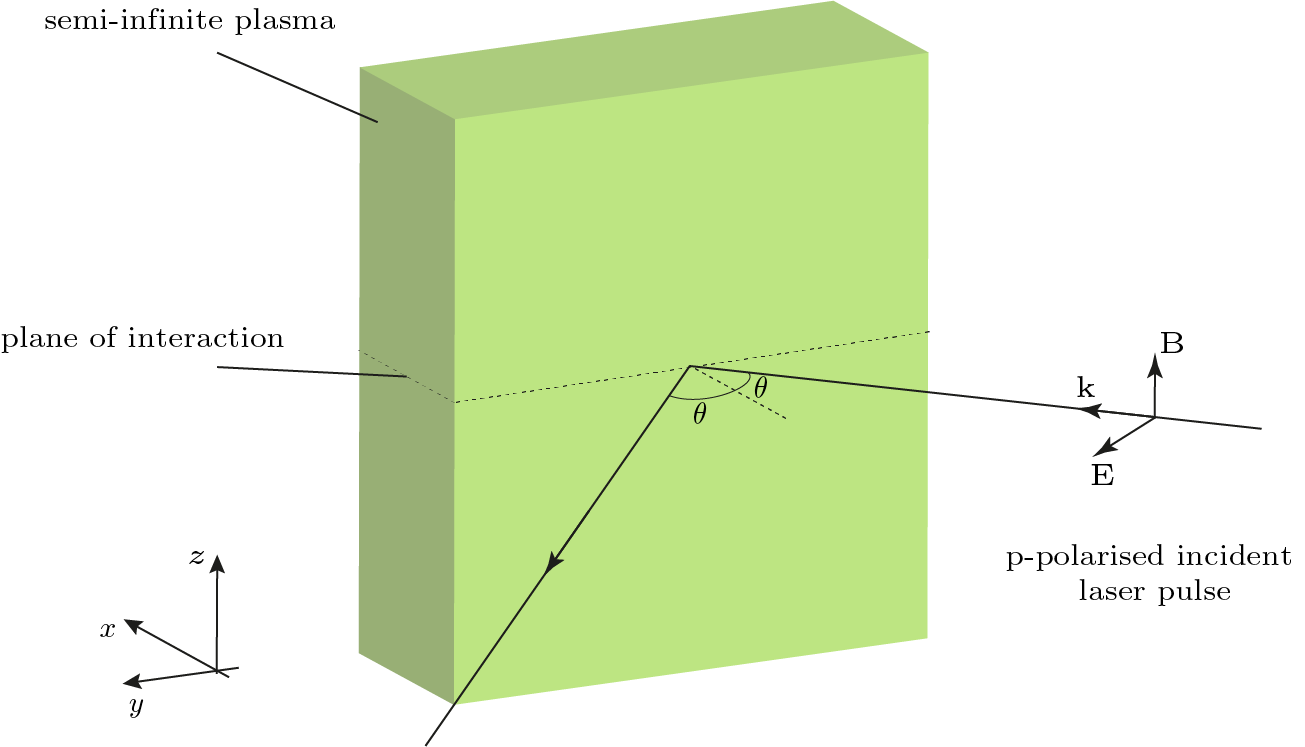
\includegraphics[width=0.7\linewidth]{figures/zvp/zvp_forces_ppol}
	\caption[Diagram of a p-polarised laser pulse incident at angle $\theta$ specularly reflected from a solid density plasma.]{Diagram of a p-polarised laser pulse incident at angle $\theta$ specularly reflected from a solid density plasma. By considering the Lorentz force equation, it is clear that all forces and therefore all plasma particle dynamics are confined to a plane.}
	\label{fig:zvpforcesppol}
\end{figure}
The Hamiltonian of a single electron confined within the potential well \cite{goldsteinClassicalMechanics2013} is
\begin{equation}\label{eq:hamiltonian_general}
	\mathcal{H} = c\sqrt{m^2_\mathrm{e}c^2 + |\mathbf{p}|^2} - e\Phi.
\end{equation}
Here, the second term of equation \ref{eq:hamiltonian_general} describes the contribution to the electron's energy from the electrostatic potential, $\Phi$, of the pseudo-capacitor. The first term is the electron energy, $U$, extracted from the invariant of the relativistic 4-momentum of the electron, $\mathbf{P^\mu} = (U/c, \mathbf{p})$,
\begin{equation}
	\mathbf{P^\mu \cdot P_\mu} = \frac{U^2}{c^2} - |\mathbf{p}|^2 = m^2_\mathrm{e}c^2.
\end{equation}
Note that while there has been growing interest in the curvature of spacetime by relativistic lasers \textbf{[cite edward here]}, for modern high power lasers, this effect remains undetectable. Thus, throughout this thesis the inner product of 4-vectors is defined using the Minkowski Metric \cite{steaneRelativityMadeRelatively2012}.

Decomposing the electron's 3-momentum into orthogonal components: $p_\mathrm{prop}$, along the laser propagation direction, $p_\mathrm{pol}$, along the polarisation axis of the laser pulse and $p_\perp$, perpendicular to both, there are two simplifications to be made. Firstly, by canonical conservation of transverse momentum, $p_\mathrm{pol} = eA$, where $A$ is the laser vector potential amplitude. Secondly, in the case of a p-polarised laser pulse (the known optimum for ZVP electron bunch generation \cite{savinAttosecondscaleAbsorptionExtreme2017} and \ac{HHG} \cite{baevaTheoryHighorderHarmonic2006}), with reference to figure \ref{fig:zvpforcesppol} and the Lorentz force law, the forces at play confine the electron trajectory to the  $p_\mathrm{prop}$-$p_\mathrm{pol}$ plane and the essential interaction geometry is two-dimensional. This is provided one considers length scales much smaller than the focal spot of the laser pulse on the target thus pondermotive pressure is normal to the target surface.

Explicitly, the Hamiltonian can be written as
\begin{equation}\label{eq:hamiltonian_specific}
	\mathcal{H} = c\sqrt{m^2_ec^2 + p^2_\mathrm{prop} + e^2A^2} - e\Phi.
\end{equation}
From equation \ref{eq:hamiltonian_specific} it is clear that should the vector potential pass through zero, one of the walls of the potential well is totally suppressed, allowing electrons in the skin layer to escape the plasma, breaking adiabaticity. The necessity of vector potential zeros for this violent reconstruction of the plasma surface led Baeva \textit{et al} \cite{baevaZeroVectorPotential2011} to coin the term `Zero Vector Potential' mechanism to describe this process. Indeed, while elementary electromagnetism tells us a laser pulse will exponentially decay within a skin layer of a plasma without passing through zero, Baeva \textit{et al} \cite{baevaZeroVectorPotential2011} were able to demonstrate in \ac{PIC} simulations that for this regime, zeros do exist and do propagate through the skin layer. The explanation relies on a Doppler shift in the laser field due to the relativistic motion of the ablating plasma surface, and the mathematical formalism of this process proceeds as follows.

[I think before this point it would be good to enter in the language of electron bunches or sheaths - I will continue the dicussion assuming this concept has been introduced].

As the \ac{ZVP} mechanism is a relativistic phenomenon, it is essential to consider the laser pulse propagating through a relativistically ablating electron bunch (i.e. with some component of its velocity anti-parallel to the laser pulse propagation direction). Transforming to the rest frame of the ablating front, beyond the relativistic critical density surface, the vector potential of the laser pulse will be an evanescent wave, at the spatial centre of the laser pulse, it can be described simply by
\begin{equation}
	\mathbf{A}'_\mathrm{L}(t',r') = A'_0\cos(\omega'_\mathrm{L}t')\exp(-r'/\delta')\hat{\mathbf{r}}'_\mathrm{pol}= A'_\mathrm{L}\hat{\mathbf{r}}'_\mathrm{pol},
\end{equation}
where the primed symbols indicate that these quantities are measured in the rest frame of the expanding front, $A'_0$ is the vector potential amplitude and $\omega'_\mathrm{L}$ is the frequency of the laser pulse, $r'$ is the propagation distance of the laser into the plasma, $\delta'$ is the skin depth and $\hat{\mathbf{r}}'_\mathrm{pol}$ a unit vector defining the polarisation direction of the laser pulse. Un-primed coordinates will indicate the lab frame measurements.

[For sure include a diagram of this]

While in previous demonstrations of the vector potential zeros, it was assumed that the ablation occurs normal to plasma surface, it is now known that this ablation occurs in the specular reflection direction and it is necessary to confirm that zeros are still predicted. Consider a p-polarised laser pulse confined to the $x$-$y$ plane incident with an angle of incidence $\theta$ on an ablating overdense plasma expanding with velocity $-v_f\hat{\mathbf{x}}$ in the lab frame, as in figure \ref{fig:zvp_ablatingfront}.
% TODO: \usepackage{graphicx} required
\begin{figure}
	\centering
	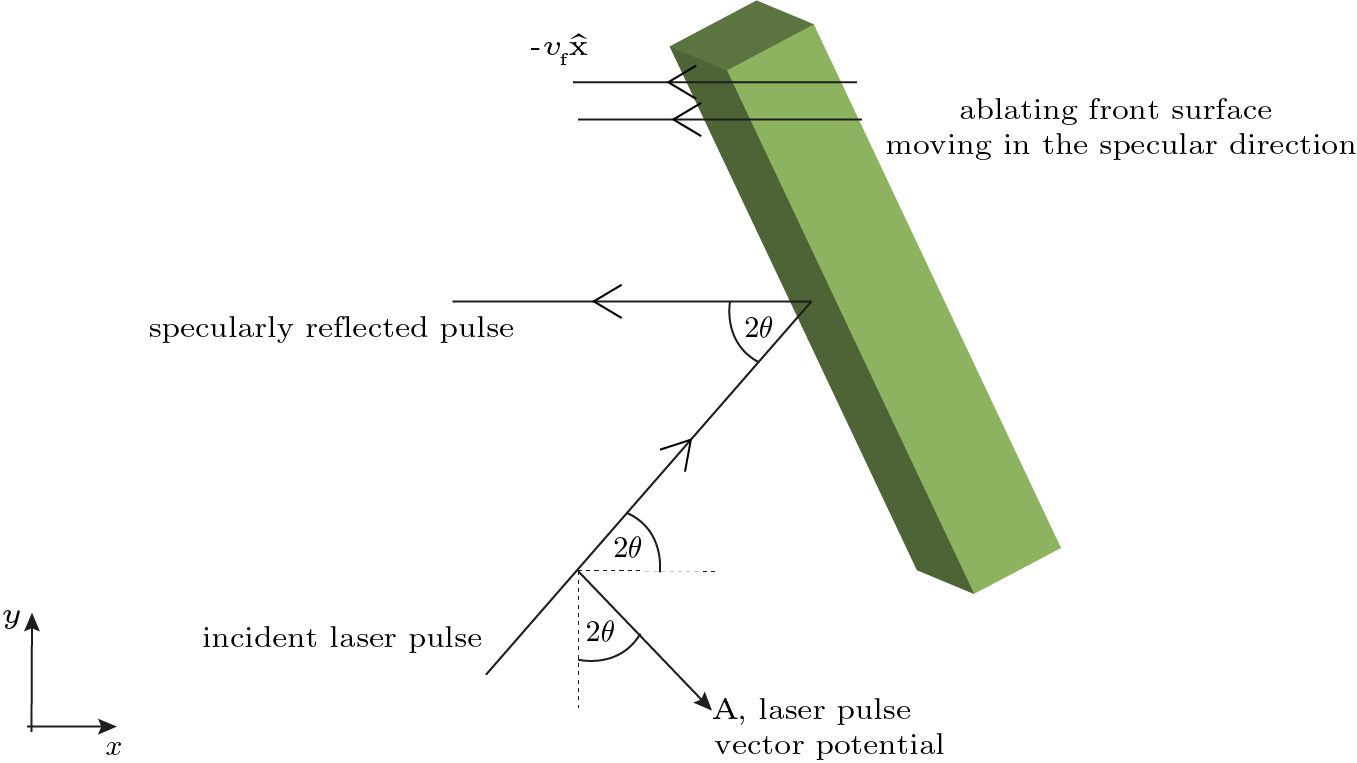
\includegraphics[width=0.7\linewidth]{figures/zvp/zvp_ablating_front}
	\caption[Diagram of a $p$-polarised laser pulse incident on an ablating overdense plasma.]{Diagram of a $p$-polarised laser pulse incident on an ablating overdense plasma. The laser is incident obliquely at an angle of $\theta$ and is reflected specularly. The plasma ablates specularly also. The interaction geometry is confined to a 2D plane.}
	\label{fig:zvp_ablatingfront}
\end{figure}
The direction of polarisation is
\begin{equation}
	\hat{\mathbf{r}}_\mathrm{pol} = \hat{\mathbf{x}}\sin{2\theta} - \hat{\mathbf{y}}\cos{2\theta}
\end{equation}
and the velocity of the rest frame of the ablating front relative to the lab frame is $-v_f\hat{\mathbf{x}}$.

Applying the Lorentz transformation to the electromagnetic 4-potential,
\begin{equation}
	\mathbf{A}_\mu = (\phi/c,\mathbf{A}),
\end{equation}
explicitly,
\begin{equation}
	\mathbf{A}'_\mu = \Lambda^\mu_\nu \mathbf{A}_\nu,
\end{equation}
where $\Lambda^\mu_\nu$, the Lorentz transform in this geometry is
\begin{equation}\label{eq:zvp_lorentz}
	\Lambda^\mu_\nu = \begin{pmatrix}
			\gamma & -\beta\gamma & 0 & 0\\
			-\beta\gamma & \gamma & 0 & 0\\
			0 & 0& 1 & 0\\
			0 & 0 & 0 & 1
	\end{pmatrix}
\end{equation}
and here $\beta = -v_\mathrm{f}/c$, $\gamma = 1/\sqrt{1-\beta^2}$. Immediately from the $y$-coordinate transformation,
\begin{equation}\label{eq:zvp_lorentz_y}
	A'_\mathrm{L}\cos{2\theta'} = A_\mathrm{L}\cos{2\theta}.
\end{equation}
Applying the headlight effect for a source moving at an angle $2\theta$ to the boosted frame,
\begin{equation}
	\cos{(2\theta')} = \frac{\cos{(2\theta)}-\beta}{1 - \beta\cos{(2\theta)}}
\end{equation}
and rearranging equation \ref{eq:zvp_lorentz_y}, the vector potential in the lab frame is
\begin{equation}\label{eq:zvp_labA}
	A_\mathrm{L} = \frac{1-\beta \sec{(2\theta)}}{1 - \beta\cos{(2\theta)}} A'_0\cos{(\omega'_L t')}\exp{(-r'/\delta')}.
\end{equation}
Writing the boosted frame space-time coordinates in terms of the lab frame coordinates,
\begin{equation}
	ct' = \gamma(ct-\beta x),
\end{equation}
\begin{equation}
	x' = \gamma(x-\beta ct),
\end{equation}
yields
\begin{equation}\label{eq:zvp_labAfull}
	A_\mathrm{L} =  A_0\cos{(\omega_L t - kx)}\exp{\left(-\frac{\sqrt{(x-\beta ct)^2+(y/\gamma)^2}}{\delta}\right)},
\end{equation}
where
\begin{equation}
	A_0 = \frac{1-\beta \sec{(2\theta)}}{1 - \beta\cos{(2\theta)}}A'_0,
\end{equation}
\begin{equation}
	\omega_L = \gamma \omega'_L,
\end{equation}
\begin{equation}
	k = \frac{\beta \gamma\omega'_L}{c},
\end{equation}
\begin{equation}
	\delta = \frac{\delta'}{\gamma}.
\end{equation}
The oscillatory term in equation \ref{eq:zvp_labAfull} demonstrates the propagation of vector potential zeros within the plasma target. From the structure of this term it would appear that these zeros are expelled from the plasma along the specular direction at a speed (recall beta is negative - change this earlier in the theory so that that negative sign is more explicit in the result.)
\begin{equation}
	v_\phi = \frac{\omega_L}{k} = \frac{c}{\beta} = -\frac{c^2}{v_\mathrm{f}}.
\end{equation}
Could also discuss here about how relativistic similarity theory derives that zeros move at speed c but how that cannot be valid since then we would always have infinitely thin radiation pulses, unless there is an extended range of zero? I suppose there is some radiation happening around the peak? Good questions..
One remaining consideration is we require that the zero gets through the whole electron bunch which is generally at very high density but is also very thin, in a way is this skin depth not what precisely determines the bunch width? The bunch will be compressed until the skin depth goes to zero across it perhaps? Things to think about.


Qualitatively, and in summary, for sufficiently intense laser pulses, electrons on the radiated surface of a solid target are accelerated by the laser to relativistic velocities at a fraction of a laser pulse cycle and therefore electrons both follow similar trajectories and are able to respond adiabatically to the $\mathbf{J}\times \mathbf{B}$ force of the laser pulse. They therefore form a high charge density thin coherent electron sheath on the front surface of the plasma but displaced inwards from the immobile ions (ions are approximately immobile on the timescale of a laser pulse cycle) via the ponderomotive pressure of the laser. This charge separation generates a longitudinal electrostatic pseudocapacitor field that confines electrons to a potential well on the front surface of the plasma, preventing further propagation of the electron bunch into the plasma bulk. When the zero of the vector potential passes through the electron bunch, the ponderomotive pressure instantaneously vanishes and electrons are ejected specularly from the target, copropagating with the zeroes and gaining energy as they discharge the pseudocapacitor field. Coherent sychrotron emission occurs concurrently. The electron bunch is then rotated by the laser pulse and launched into the bulk at high energy.


SOmething to think about: which comes first? electron bunch acceleration across pseudo capacitor or zeros?
Laser accelerates electorns in laser propagation direction , however cannot propagate further into the plasma so only get motion parallel to surface, once potentail well disrupted, accleration is perp to surface so combined, electrons travel in specular direction.
So actually what we are saying is the zeros will go in whatever direction the surface ablates in, but the surface will move in a direction dependent on the components of electron 


\subsubsection{The headlight effect}\label{sec:zvp_headlight}
This most likely goes in the appendix. But storing here for now.

The headlight effect describes the beaming of an isotropically emitting source travelling at some velocity relative to an observer. Consider the geometry of figure \ref{fig:zvp_ablatingfront} with the source (the laser pulse) travelling at an angle $2\theta$ to the observer (in this case, the ablating front). A photon with energy $E$ emitted from the rest frame of the source (in this case the lab frame) has a 4-momentum
\begin{equation}
	\mathbf{P}_\mu = \left(\frac{E}{c},\frac{E}{c}\cos{2\theta},\frac{E}{c}\sin{2\theta}\right).
\end{equation}
As the interaction geometry is confined to a 2D plane,  the $z$-component can be safely neglected. Applying the lorentz boost of equation \ref{eq:zvp_lorentz},
\begin{equation}
	\begin{split}
		\frac{E'}{c} = \gamma \left( \frac{E}{c} - \beta \frac{E}{c}\cos{2\theta}\right) \\
		\frac{E'}{c}\cos{2\theta'} = \gamma \left( \frac{E}{c}\cos{2\theta} - \beta \frac{E}{c}\right).
	\end{split}
\end{equation}
Solving these equations for the angle in the boosted frame,
\begin{equation}
	\cos{2\theta'} = \frac{\cos{2\theta} - \beta}{1-\beta\cos{2\theta}}.
\end{equation}

\subsubsection{Conservation of generalised transverse momentum}\label{sec_app_conservation-generalised-mometum}
This should most likely go in the appendix/ before ZVP Hamiltonian discussion.

Whilst it is commonly stated within the field of laser-solid interactions, it would appear that some nuance/detail is missing from the discussion which in turn shrouds the \ac{ZVP} mechanism in confusion.

Consider a holonomic system of N relativistic particles under the influence of electromagnetic forces. A particle $j$ with charge $e_j$ and mass $m_\mathrm{j}$ experiences a scalar potential,
\begin{equation}
	U_{j} = e_j(\Phi - \mathbf{A} \cdot \mathbf{v}_{j})
\end{equation}
and hence the system is described by the Lagrangian
\begin{equation}
	L = \sum^N_{j=1}\left( - m_\mathrm{j}c^2\sqrt{1-\beta^2_\mathrm{j}} - e_j(\Phi - \mathbf{A} \cdot \mathbf{v}_\mathrm{j}) \right),
\end{equation}
where $\beta^2 = \mathbf{v}_\mathrm{j}\cdot\mathbf{v}_\mathrm{j} /c^2$ \cite{goldsteinClassicalMechanics2013}.
The generalised momentum corresponding to coordinate $x_j$ is
\begin{equation}
	p_{j,x} = \frac{\partial L}{\partial \dot{x}_j} = m_j\dot{x}_j + e_jA_x,
\end{equation}
explicitely, the generalised momentum describes both the linear mechanical momentum and the momentum of the electromagnetic field. Via Noether's theorem, if $L$ is independent of $x_j$, \textit{i.e.} spatially homogeneous along $x$ for particle $j$, then 
\begin{equation}
	\dot{p}_{j,x} = 0.
\end{equation}
Considering a p-polarised Gaussian laser pulse, axis of polarisation along $x$, $A_x$ will be approximately constant. Integrating and noting that initially there is no linear or electromagnetic momentum, the generalised transverse momentum conservation equation for an electron at the plasma-vacuum boundary is obtained, namely,
\begin{equation}
	p_\mathrm{T} = eA,
\end{equation}
where $p_mathrm{T}$ is the electron momentum along the polarisation axis of the laser pulse. and $A$ its vector potential.

Note that this is only valid provided the radiating electron does not radiate along the direction of $\mathbf{A}$ as discussed by Sokolov \textit{et al} \cite{sokolovDynamicsEmittingElectrons2009}. But we do know this radiation is specular so this is true for normal incidence but not specular?? Really need to consider what the EM fields are in the surface from combined Incident and reflected.
The implications of this should maybe be considered?? Also note that this is only true for gaussian pulses with spatial profiles $\gg$ than electron trajectories (\textit{i.e.} twice the relativistic larmor radius).

\subsection{ZVP electron bunch energies}\label{sec:zvp_energies_derivation}
In \cite{baevaZeroVectorPotential2011}, Baeva \textit{et al} propose energy scalings for electron bunches produced in the \ac{ZVP} regime as a function of the laser intensity and plasma density, finding that one of the key statements of similarity theory ($p \sim a_0 S^x$, where $x$ is some integer value, THIS NEEDS A CITE I THINK IT APPEARS IN BAEVAS ORIGINAL HHG PAPER) holds for the \ac{ZVP} mechanism. Later this was then extended to \ac{3D} by Savin \textit{et al} \cite{savinAttosecondscaleAbsorptionExtreme2017}. What follows is that discussion with a more close consideration of the both consequences and constants of proportionality.

(Pherhaps I should redo this discussion condering infinitessimal areas of the plasma surface to show how variation can exist across the surface) Defo do this! And say that provided the variation is small, rel to what though? the surface remains approximately flat -> that is totally not true

Consider again the semi-infinite block of plasma proposed in figure \ref{fig:zvp_ablatingfront}, normally irradiated by a laser pulse with wavelength $\lambda_\mathrm{L}$ and peak electric field, $E_\mathrm{L}$. It is now the ponderomotive pressure of the laser that displaces the electron fluid. Consider ust one laser cycle. The electron surface moves inwards until the pressure exerted by the peak instantaneous ponderomotive pressure of the laser pulse cycle,
\begin{equation}
	\mathbf{P}_\mathrm{L} = \epsilon_0 E^2_\mathrm{L} \hat{\mathbf{x}} = \epsilon_0 \left(\frac{a_0\omega_\mathrm{L}m_\mathrm{e}c}{e}\right)^2 \hat{\mathbf{x}}
\end{equation}
is equal and opposite to the pressure exerted by the pseudo-capacitor field,
\begin{equation}
	\mathbf{P}_\mathrm{C} = \frac{QE}{\sigma} \hat{\mathbf{x}}= -\frac{(en_\mathrm{e}\Delta x)^2}{\epsilon_0}\hat{\mathbf{x}}
\end{equation} 
using equations \ref{eq:intro_Q} and \ref{eq:intro_E}. Equating the magnitudes of $\mathbf{P}_\mathrm{L}$ and $\mathbf{P}_\mathrm{C}$, the maximum displacement inwards of electrons is
\begin{equation}\label{eq:zvp_dx}
	\Delta x \hat{\mathbf{x}} = \frac{c}{\omega_\mathrm{L}}\frac{a_0}{\bar{n}_\mathrm{e}}\hat{\mathbf{x}}  = \frac{1}{kS}\hat{\mathbf{x}},
\end{equation}
where $k$ is the wave-vector of the laser pulse. Correspondingly,
\begin{equation}\label{eq:zvp_E}
	E = \frac{en_\mathrm{e}}{\epsilon_0}\Delta x = \frac{\omega_\mathrm{L}cm_\mathrm{e}a_0}{e} = E_\mathrm{L}.
\end{equation}
Applying the results of equations \ref{eq:zvp_dx} and \ref{eq:zvp_E}, when the ponderomotive pressure vanishes and the electron bunch is launched across the pseudo-capacitor, the relativistic kinetic energy gained by a single electron is
\begin{equation}\label{eq:zvp_T}
	T =  \int \mathbf{F}\cdot\mathrm{d}\mathbf{s} = \int^0_{\Delta x} -eEdx = \int^0_{\Delta x}-\frac{en_\mathrm{e}x}{\epsilon_0}dx = \frac{1}{2}m_\mathrm{e}c^2\frac{a^2_0}{\bar{n}_\mathrm{e}}
\end{equation}
or an electron gamma factor,
\begin{equation}
	\gamma = \frac{1}{\sqrt{1-\beta^2}} = 1 + \frac{a_0^2}{2\bar{n}_\mathrm{e}}.
\end{equation}
Assuming all displaced electrons are captured by the pseudo-capacitor field and launched as a coherent bunch, the total number of electrons in the bunch is
\begin{equation}\label{eq:zvp-Ne}
	N_\mathrm{e} = n_\mathrm{e} \sigma \Delta x = \frac{\sigma a_0 n_\mathrm{c}}{k}  = \sigma \epsilon_0 E_\mathrm{L}
\end{equation}
and hence, the total kinetic energy of the electron bunch is
\begin{equation}\label{eq:zvp_U}
	U_\mathrm{ZVP} = N_\mathrm{e} T = \frac{\sigma n_\mathrm{c}}{k}\times \frac{1}{2}m_\mathrm{e}c^2 \frac{a^3_0}{\bar{n}_\mathrm{e}}.
\end{equation}
It is now interesting to compare equation \ref{eq:zvp_U} to the laser energy deposited upon the plasma surface and therefore consider what fraction of the laser energy can be absorbed via the \ac{ZVP} mechanism. Using $E = E_\mathrm{L}$, \ref{eq:zvp_U} can be rewritten as
\begin{equation}
	U_\mathrm{ZVP} = \frac{1}{2\omega_\mathrm{L} S}\sigma c \epsilon_0 E^2_\mathrm{L}.
\end{equation}
For the case of normal incidence, bunches are produced at a frequency of $2\omega_\mathrm{L}$, naturally following the frequncy of the $\mathbf{J}\times \mathbf{B}$ force. Assuming a sinusoidal plane wave incident with surface area $\sigma$, the energy absorbed in half a laser cycle is
\begin{equation}
	 U_\mathrm{L,1/2} = \sigma \frac{T}{2}\langle I_\mathrm{L}\rangle = \frac{2\pi}{4\omega_\mathrm{L}}\sigma c\epsilon_0E^2_\mathrm{L}.
\end{equation}
Hence,
\begin{equation}
	\eta_\mathrm{ZVP} = \frac{U_\mathrm{ZVP}}{U_\mathrm{L,1/2}} = \frac{1}{\pi S}.
\end{equation}
Interestingly, this new analytical result predicts the trend observed by A. Savin \cite{savinModellingLaserPlasmaInteractions2019} in \ac{PIC} simulations both in magnitude and in scaling. Indeed, A. Savin demonstrated 
\begin{equation}
	\eta_\mathrm{ZVP} \sim S^{-1.000(3)},
\end{equation}
however, this result led A. Savin to conclude increasing $S$ increases the energy in the reflected \ac{HHG} beam thus increasing high harmonic efficiency, seemingly in tension with the vast majority of the work on this regime [CITE CITE CITE]. The resolution arises from the follwoing: there are two distinct conversion efficiencies which describe the reflected harmonic spectrum: the conversion efficiency into the whole reflected beam and the conversion efficiency into individual harmonics. While the total conversion into the reflected beam decreases for decreasing $S$, the slope of the harmonic spectrum also decreases and therefore while A. Savin is absolutely correct, the imporant parameter (the slope of the harmonic spectra) follows the opposite trend.

Indeed high X-ray harmonic efficiency neccesitates high inefficiencies in the production of ZVP electron bunches as higher energy bunches produce more coherent reflected radiation, a caveat not often considered in the quest for higher-order harmonics.


[Side note for my reference: bunch is made and at peak compression at peak of laser pulse. then laser field oscillates,inside the bunch they experience an a0 = 0(? maybe) outside there is a minimum in the field, then the bunch is rotated back when it hits the next peak of the laser pulse (ie a0=0? outside plasma?) the upshot of this is I can then say there is a distance of lambda/2 between bunch peak displacement and radiation point and since peak displacement = 1/kS, for all S, the pseudocapacitor has been completely discharged and therefore there has been the maximum energy gain before HHG production - important for electron bunch gamma factor discusion.]


Next up: the unification of RES and ZVP.

\subsection{ZVP bunches oblique incidence scaling and internal bunch structure}
This section is inspired by \cite{gonoskovUltrarelativisticNanoplasmonicsRoute2011} and \cite{vincentiOpticalPropertiesRelativistic2014} supplementary material but different where I believe they have gone wrong to generalise the \ac{ZVP} mechanism energy scalings.

The below section needs cleaning up of minus signs etc, take the convention laser propagates in the positive direction therefore drift of electrons and ions in frame with normal incidence is in negative direction.

As has previously been stated, if the plasma-vacuum boundary is sufficiently steep, the plasma electrons will respond adiabatically to the laser pulse and arrange themselves to form a pseudocapacitor longitudinal electric field $E_\mathrm{C}$ at the plasma surface. At all points in this adiabatic phase, the surface electrons will be in a quasi-static equilibrium \textit{i.e.} there will be a balance between the electromagnetic forces on them. Consider again a laser pulse incident on a solid density plasma existing for $x>0$ at angle $\theta$. Transforming to the reference frame where the laser is incident normally (quantities in this frame are indicated by the primed symbol), the electron and ion bulk plasma species are now streaming with a velocity $\mathbf{v}_\mathrm{d} = -c \sin\theta \hat{\mathbf{y}}$.  From the Lorentz force law along the longitudinal direction ($\hat{\mathbf{x}}$), for a displacement of the electron fluid $x'_\mathrm{e}$ (one assumes that the expression for a single electron at the surface describes the surface as via relativity all electrons follow similar trajectories), travelling at speed $\mathbf{v'}$
\begin{equation}\label{eq:zvp_eq}
	-e(\mathbf{v'}(x'_\mathrm{e})\times (\mathbf{B}'_\mathrm{L}(x'_\mathrm{e}) + \mathbf{B}'_\mathrm{i}(x'_\mathrm{e}))\cdot \hat{\mathbf{x}} + E'_\mathrm{C}(x'_\mathrm{e}) )= 0,
\end{equation}
where 
\begin{equation}\label{eq:zvp_Bl}
	B'_\mathrm{L} = \frac{m_\mathrm{e} \omega'_\mathrm{L}a_0\sin(\omega'_\mathrm{L}t'-k'x'_\mathrm{e})}{e} \hat{\mathbf{z}}
\end{equation}
and $B_\mathrm{i}$ originates from the uncompensated ion current, $\mathbf{J_\mathrm{i}} =  Zen'_\mathrm{i}(x'_\mathrm{e}) \mathbf{v}_\mathrm{d}$, where the electron fluid has been displaced. As before, from equation \ref{eq:intro_E},
\begin{equation}\label{eq:zvp_Ec}
	E'_\mathrm{C} = \frac{en'_\mathrm{e}x'_\mathrm{e}}{\epsilon_0}.
\end{equation}
Note that there is no contribution to the laser magnetic field here from the reflected laser pulse since the assumption is that during this pushing phase all laser pulse energy is converted into electrostatic potential energy, this is supported by the attosecond duration of the reflected harmonic beam (\textit{i.e.} it is not produced during this phase). Maxwell-Ampère's Law states
\begin{equation}\label{eq:zvp_maxwellampere}
	\nabla \times \mathbf{B} = \mu_0 \mathbf{J}.
\end{equation}
Noting that by symmetry there can be no variation in the magnetic field with $y'$ or $z'$ it becomes clear that
\begin{equation}\label{eq:zvp_BiJi}
	-\frac{\mathrm{d}(\mathbf{B}'_\mathrm{i})_{z'}}{\mathrm{d} x'} = \mu_0 (\mathbf{J}_\mathrm{i})_{y'}.
\end{equation}
Integrating equation \ref{eq:zvp_BiJi} from $-\infty$ to $x'_\mathrm{e}$, noting that $\mathbf{B}_\mathrm{i} = 0$ at infinity and assuming a constant density profile $n'_\mathrm{i}$ for $x>0$,
\begin{equation}\label{eq:zvp_Bi}
	\mathbf{B}'_\mathrm{i}(x'_\mathrm{e}) = \mu_0 en'_\mathrm{e}x'_\mathrm{e}c\sin(\theta)\hat{\mathbf{z}}.
\end{equation}
Using equations \ref{eq:zvp_Bl}, \ref{eq:zvp_Ec} and \ref{eq:zvp_Bi} and making the very reasonable approximation that the relativistic electrons on the surface move at speed $v'_y \approx \pm c$ at peak displacement ($x'_\mathrm{e} = x'_\mathrm{p}$), \ref{eq:zvp_eq} can be written as
\begin{equation}
	-e\left(\pm c\left(\pm\frac{m_\mathrm{e}\omega'_\mathrm{L}a_0}{e} + \mu_0 en'_\mathrm{e} x'_\mathrm{p}c\sin\theta\right)+\frac{en'_\mathrm{e}x'_\mathrm{p}}{\epsilon_0}\right) = 0.
\end{equation}
Note that to be in the laser pushing phase the first term must be negative, corresponding to $\mathbf{v'}$ and $\mathbf{B}'_\mathrm{L}$ having the opposite sign, hence,
\begin{equation}
	 c\left(-\frac{m_\mathrm{e}\omega'_\mathrm{L}a_0}{e} \pm \mu_0 en'_\mathrm{e} x'_\mathrm{p}c\sin\theta\right)+\frac{en'_\mathrm{e}x'_\mathrm{p}}{\epsilon_0} = 0,
\end{equation}
where here the $\pm$ tracks the sign of $\mathbf{v}'$. After some maniputation, one arrives at
\begin{equation}
	x'_\mathrm{p} = \frac{1}{k'S' (1\pm \sin\theta)}.
\end{equation}
Transforming back to the lab frame, naturally,
\begin{equation}
	x_\mathrm{p} = \frac{1}{kS(1\pm \sin\theta)}.
\end{equation}
Already this is quite a result, reducing to equation \ref{eq:zvp_dx} for $\theta =0$ and predicting the suppression and enhancement of the two surface oscillations per laser puse cycle. Explicitely, for a laser pulse propagating at $y = x\tan\theta$, the peak displacement of the electron surface is enhanced for $\mathbf{B}_\mathrm{L}$ in the $+\hat{\mathbf{z}}$-direction and suppressed for $\mathbf{B}_\mathrm{L}$ in the $-\hat{\mathbf{z}}$-direction.

Consider now acceleration of the electron bunch across the pseudocapacitor field in the boosted frame,
\begin{equation}\label{eq:zvp_Tp}
	T' = \int \mathbf{F}'\cdot \mathrm{d} \mathbf{s}' = \int^0_{x'_\mathrm{p}} -eE'_\mathrm{C}(x'_\mathrm{e}) \mathrm{d}x'_\mathrm{e} =  \frac{en'_\mathrm{e}(x'_\mathrm{p})^2}{2\epsilon_0}=\frac{1}{2}m_\mathrm{e}c^2\frac{a^2_0}{\bar{n}'_\mathrm{e}(1\pm \sin\theta)^2}.
\end{equation}
Again, transforming back to the lab frame, noting the gain in energy from crossing the pseudo-capacitor 


The linearity of four-vectors ensures 
\begin{equation}
	\mathbf{\Delta P}^\mathrm{\mu} = (\frac{\Delta E}{c}, \mathbf{\Delta p})
\end{equation}
is also a four-vector. The Lorentz transform for change in energy is thus
\begin{equation}
	\Delta E = \gamma \left(\Delta E' - \frac{\mathbf{v}_\mathrm{d}}{c}\cdot \mathbf{\Delta p'}\right),
\end{equation}
where 
\begin{equation}\label{eq:zvp_gamma}
	\gamma = \frac{1}{\sqrt{1+\sin^2\theta}} = \frac{1}{\cos\theta}.
\end{equation}
Hence for energy gain $\Delta E' = T'$ in the boosted frame (where $\Delta p_y = 0$),
\begin{equation}
	T = \gamma T'.
\end{equation}
Using equations \ref{eq:zvp_Tp} and \ref{eq:zvp_gamma} and recalling $\bar{n}_\mathrm{e} = \bar{n}'_\mathrm{e}/\gamma$,
\begin{equation}\label{eq:zvp_Tzvp_theta}
	T =m_\mathrm{e}c^2 \frac{a_0}{2S(1\pm\sin\theta)^2}
\end{equation}
Nb this could have simply been established in the lab frame and considering F.ds which is just the same[The electron bunch then accelerates across the pseudo-capacitor in the specular direction, the force ] maybe put this derivation in appendix.

Also note that when doing this transformation, T is the energy gained but there is another term in the momentum from the transform, since now $v_y = c\sin\theta$. This is unrelated to the energy gain from crossing the pseudo capacitor. There is no explanation of where this energy comes from, just that in order for the bunch to travel in the -x direction in the boosted frame - not sure what real explanation there is for this to occur, also confusion here since is this actually contained within the gamma expression or not, im lost come back to this. Maybe actualyl this is fine. We jsut take the gamma factor associated with the py gain ($=\sec\theta$ - corresponding to a gamma of 1.4 at 45 degrees) and add the delta gamma from the pseudo capacitor and that should be fine.

Another note: this dependence on theta ($1\pm \sin\theta$) can be explained as an increase due to the electric field having a component acting either in or out from the plasma surface either assisting or counteracting the magnetic field.

Idea: Can one use an external constant magnetic field to obtain the same results for normal incidence?

Also need to go back through this section and make clear which gamma is which in this section

Therefore, as with peak displacement, the energy gained by the electron bunch via the ZVP mechanism is suppressed in one half cycle and enhanced in the second.

While this model would suggest an optimal angle for electron energy and therefore \ac{HHG} of $\pi/2$, if $\theta > \pi/4$, then, if the relativistic electron bunch is travelling at $c$ along the specular reflection direction, the subsequent laser peak amplitude will never `catch up' with the electron bunch, and electrons will escape through the antinodes (?) of the electric field [CITE KRUSHELNICK PAPER GRAZING INCIDENCE ELECTRONS], generating high charge electron bunches in reflection, but decreasing \ac{HHG efficiency}.

Finally, moving on to the calculation of total bunch energy as a function of $\theta$. Since the total number of electrons in the accelerating bunch must be invariant,
\begin{equation}\label{eq:zvp_Uzvp_theta}
	U_\mathrm{ZVP}(\theta) = n_\mathrm{e}\sigma\Delta x T(\theta) =  \frac{\sigma n_\mathrm{e}}{k}\times m_\mathrm{e}c^2\frac{a_0}{2S^2(1\pm \sin\theta)^3}.
\end{equation}
What we can see from this is this enables a larger fraction of the laser energy to be absorbed at high $S$ pushing the currently experimentally accessible regime into the most efficient regime.

I want to move on, but return to this section and sort out the following. 


Another concern: peter showed me sims that suggested that increasing S incerased the suppressed oscillations more RELATIVE to the main oscilisations, perhaps need to look at the internal bunch structure?

Also see if can do a second order calculation through the electron bunch to see if can calculate its structure.



Big note:
The highest electron gamma factors comes from those electrons at the very front surface who are accelerated before high density is reached and quasistatic equilibrium reached (there are therefore very few of them), these few electrons do not satisfy ZVP relation for energy, instead 
ponderomotvie + ZVP which at most would be twice the predicted gamma which is quite some difference HOWEVER for all experiments so far, ZVP energy gain is small since S large so ponderomotive is more sensible.



Earlier write something along the lines of explaining while ZVP absorption does represent laser energy absorption, bulk heating occurs rather indirectly.

\section{Defining characteristics of the ZVP mechanism}
In her original paper, T. Baeva \textit{et al} \cite{baevaZeroVectorPotential2011} outlined 6 defining characteristics of the \ac{ZVP} mechanism, namely,
\begin{enumerate}
	\item The existance of vector potential zeros moving through the skin layer in the laboratory frame;
	\item The existance of zeroes in the incident laser pulse vector potential required for the formation of fast electron bunches;
	\item The generation of fast electron bunches with ultra-short temporal duration;
	\item Such bunches should be described by the expressions for average \ref{eq:zvp_Tzvp_theta} and total energy \ref{eq:zvp_Uzvp_theta};
	\item An intrinsic link must exist between the fast electron bunches and coherent X-ray \ac{HHG};
	\item Injection of the fast electron bunches along the propagation axis of the laser pulse;
\end{enumerate}
with the essential point being it is the moving zeros within the skin layer being the defining delineator between this post-ponderomotive regime of laser pulse energy absorption and all other proposed mechanisms. While such observational requirements are far beyond the reaches of currently experimental know-how, numerical simulations in both 1- \cite{baevaZeroVectorPotential2011} and 2-dimensions \cite{savinAttosecondscaleAbsorptionExtreme2017} have confirmed the above points. Now is presented the first \ac{3D} simulations to demonstrate the \ac{ZVP} mechanism.

\section{Numerical simulations of the ZVP mechanism}
This thesis relies throughout on the analysis of 1,2 and 3D \ac{PIC} simulations, primarily using the massively-parallel and open-source simulation code Smilei \cite{derouillatSmileiCollaborativeOpensource2018}. Simulation parameters will be provided throughout.
\subsection{The ZVP mechanism in 3D}
Results are presented in figure \ref{fig:zvp3d}.

Discuss choice of S parameter somewhere. Also note that these parameters are currently accessible on ELI-NP.

\begin{figure}
	\centering
	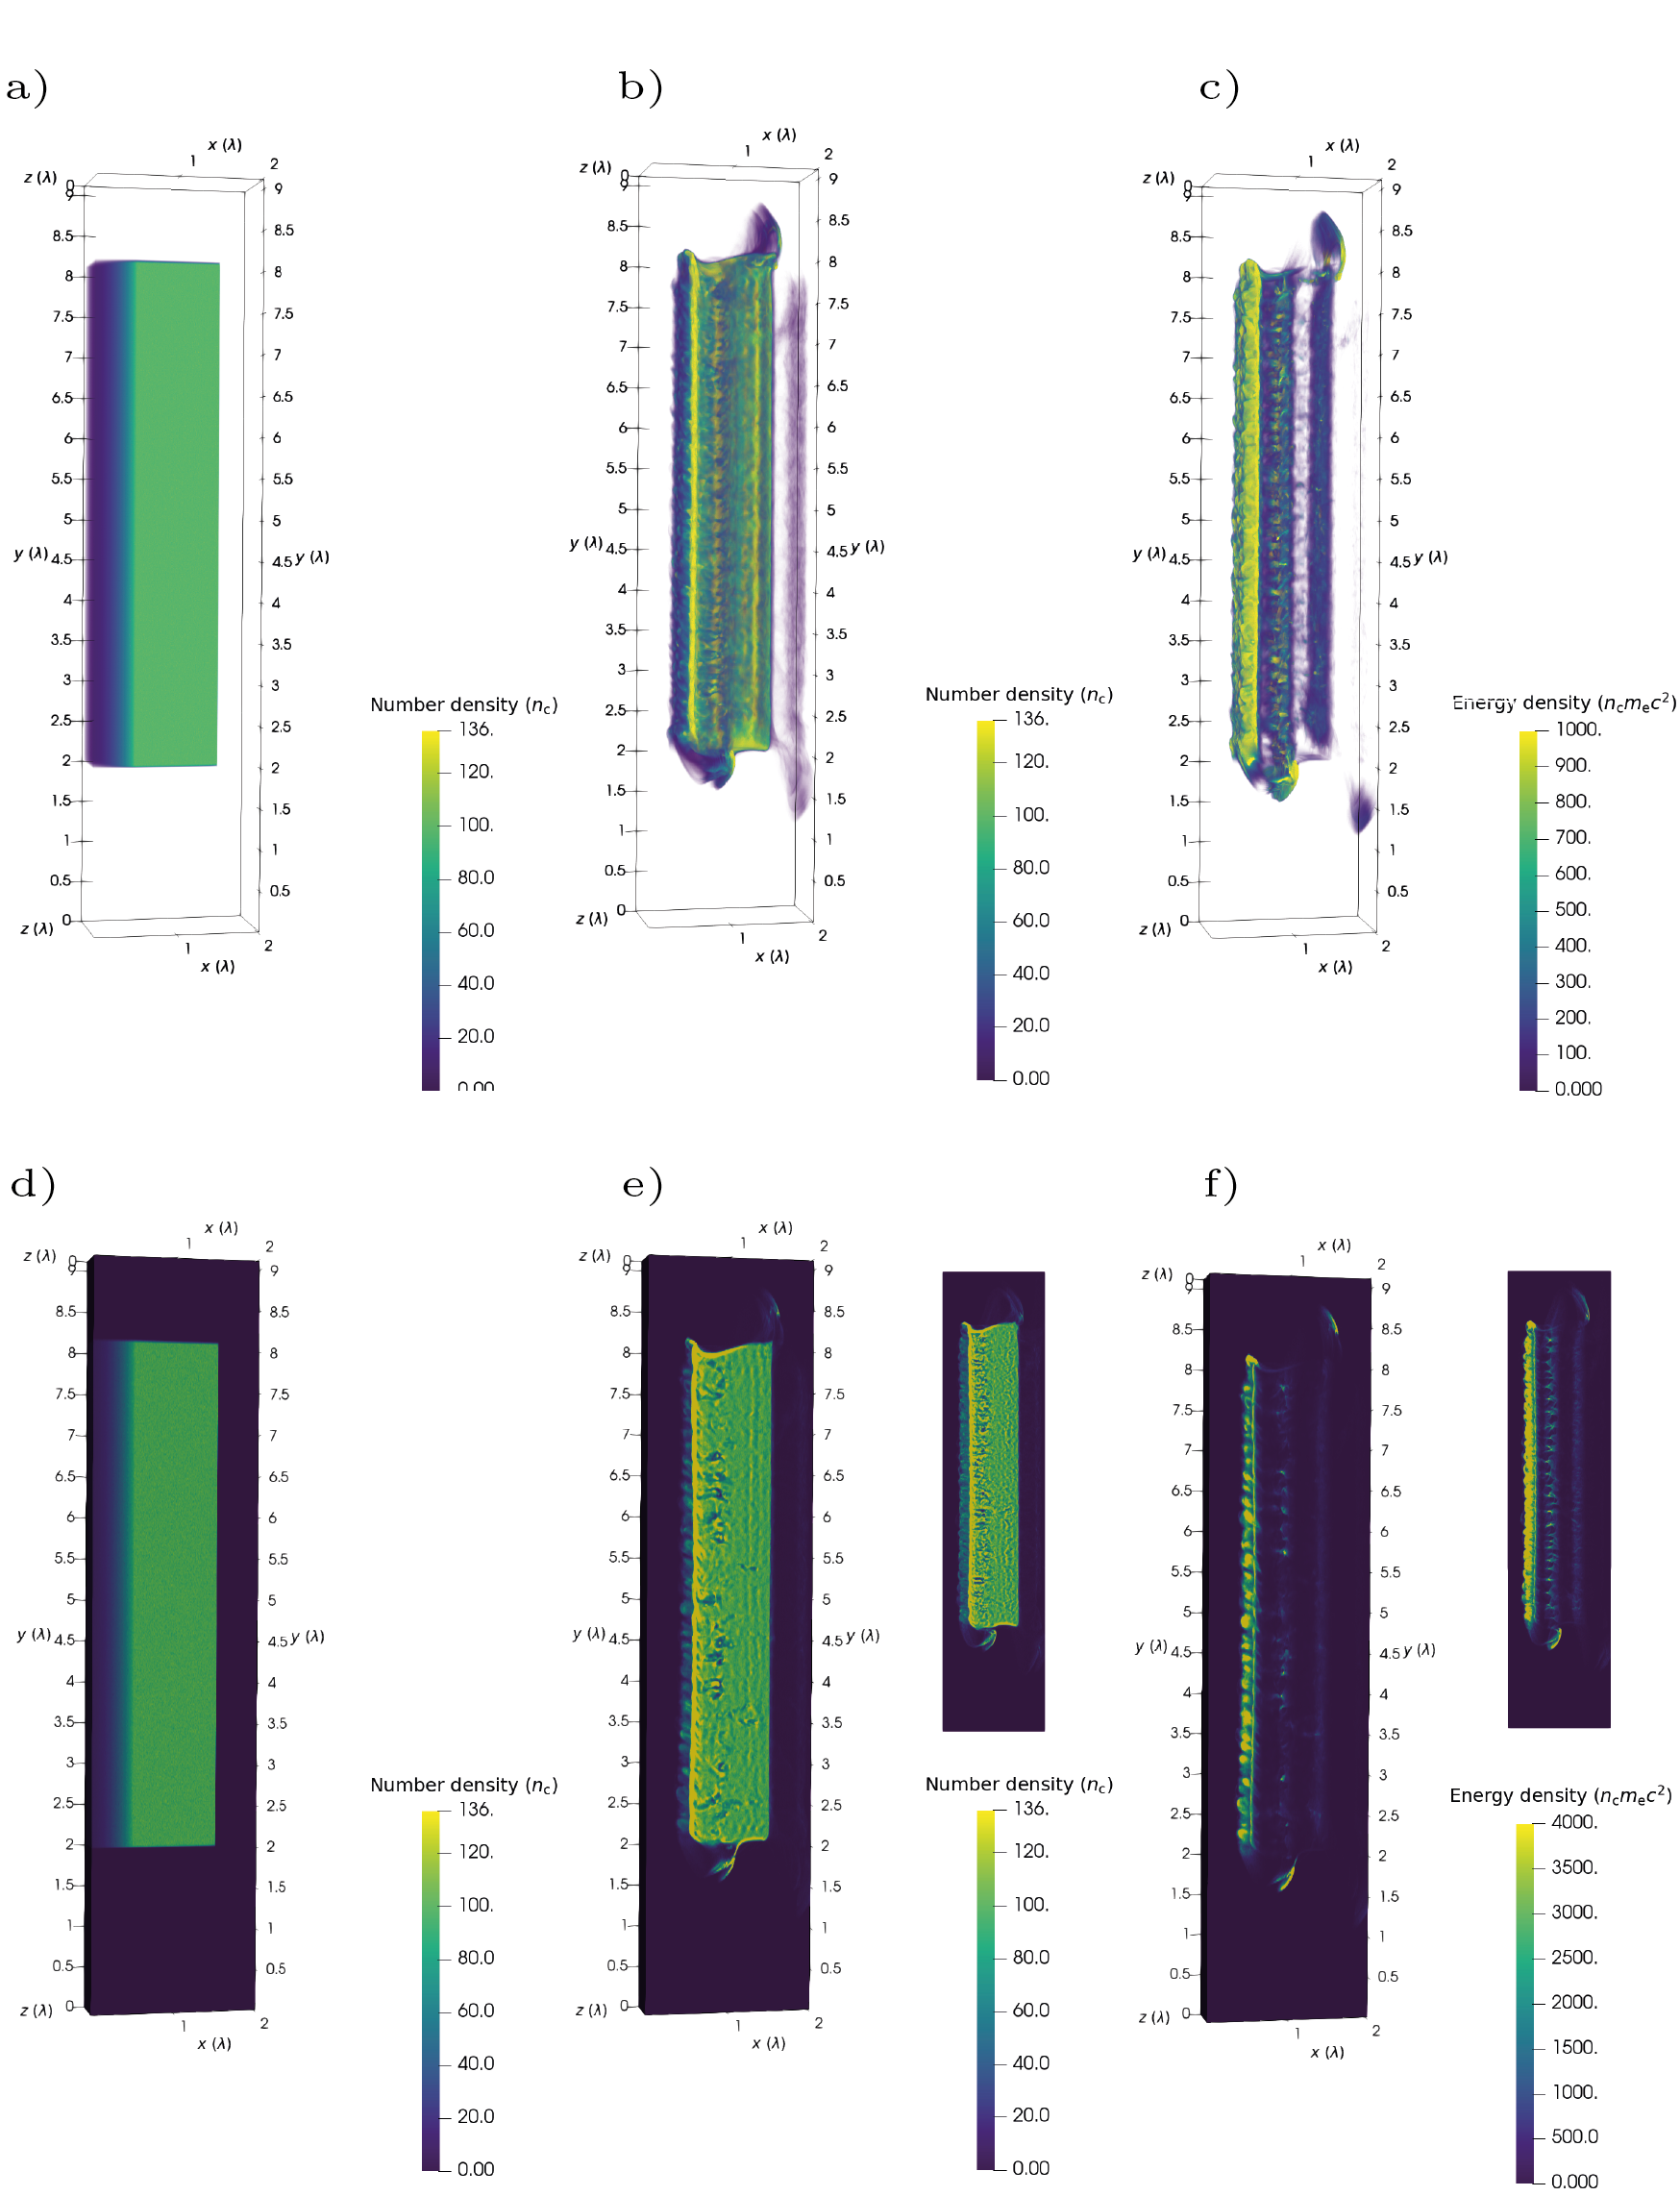
\includegraphics[width=1\linewidth]{figures/zvp/zvp_3D}
	\caption[Simulation results from a 3D \ac{PIC} simulation of the \ac{ZVP} mechanism. ]{Simulation results from a 3D \ac{PIC} simulation of the \ac{ZVP} mechanism. a) The initialised electron number density. b) The electron number density several cycles later, the plasma bulk is intact, however there is evidence of instabilities and electron bunches propagating through and around the plasma. c) The electron kinetic energy density at the same timestep. Note that the scale has been clipped to enable observation of both electron bunches propagating through and around the plasma bulk. Significantly higher energy density, corresponding to a higher charge density and attosecond duration for the electron bunches propagating around the bulk. d-f) Plots clipped through $z=0$ for a-c) respectively for better clarity on the internal structure of the plasma bulk. The accompanying plots for figures e) and f) are corresponding 2D PIC simulation results.}
	\label{fig:zvp3d}
\end{figure}
I will finish this section once the results of the rest of the 3D sim stuff is done. One thing to remark:

The remarkable similarity between the 2 and 3D simulation results is a natural consequence of the 2D nature of the interaction geometry. It is however still reassuring to note that previous work withstands this stringent test of the real universe. 

(At some point list all the other sources of potential error, including ignoring ionisation, ionisation states, collisions.)

Interesting result of the 3D sim: Can see bunch on front surface and laser clearly propagating behind it. Is this since in this new regime (ZVP dominating HHG) the thin bunch barely attenuates (ie reflects) the laser pulse when it is accelerating across the pseudo capacitor, hence the laser is still effectively able to compress the plasma surface and keep the process going. Meanwhile the reflected HHG light comes mostly from converting bunch KE into HHG.


\subsubsection{Convergence of 3D simulations}
The 3D simulation parameters were chosen to be consistent with previous work on the \ac{ZVP} mechanism, however, such simulations are cumbersome, limiting the number of simulations it is feasible to run. Certainly parameter scans are not currently available. In order to query the defining characteristics outlined by Baeva, a smaller simulation was run with similar parameters to the initial simulation (this is 9/18compare) but at lower resolution. 
% TODO: \usepackage{graphicx} required
\begin{figure}
	\centering
	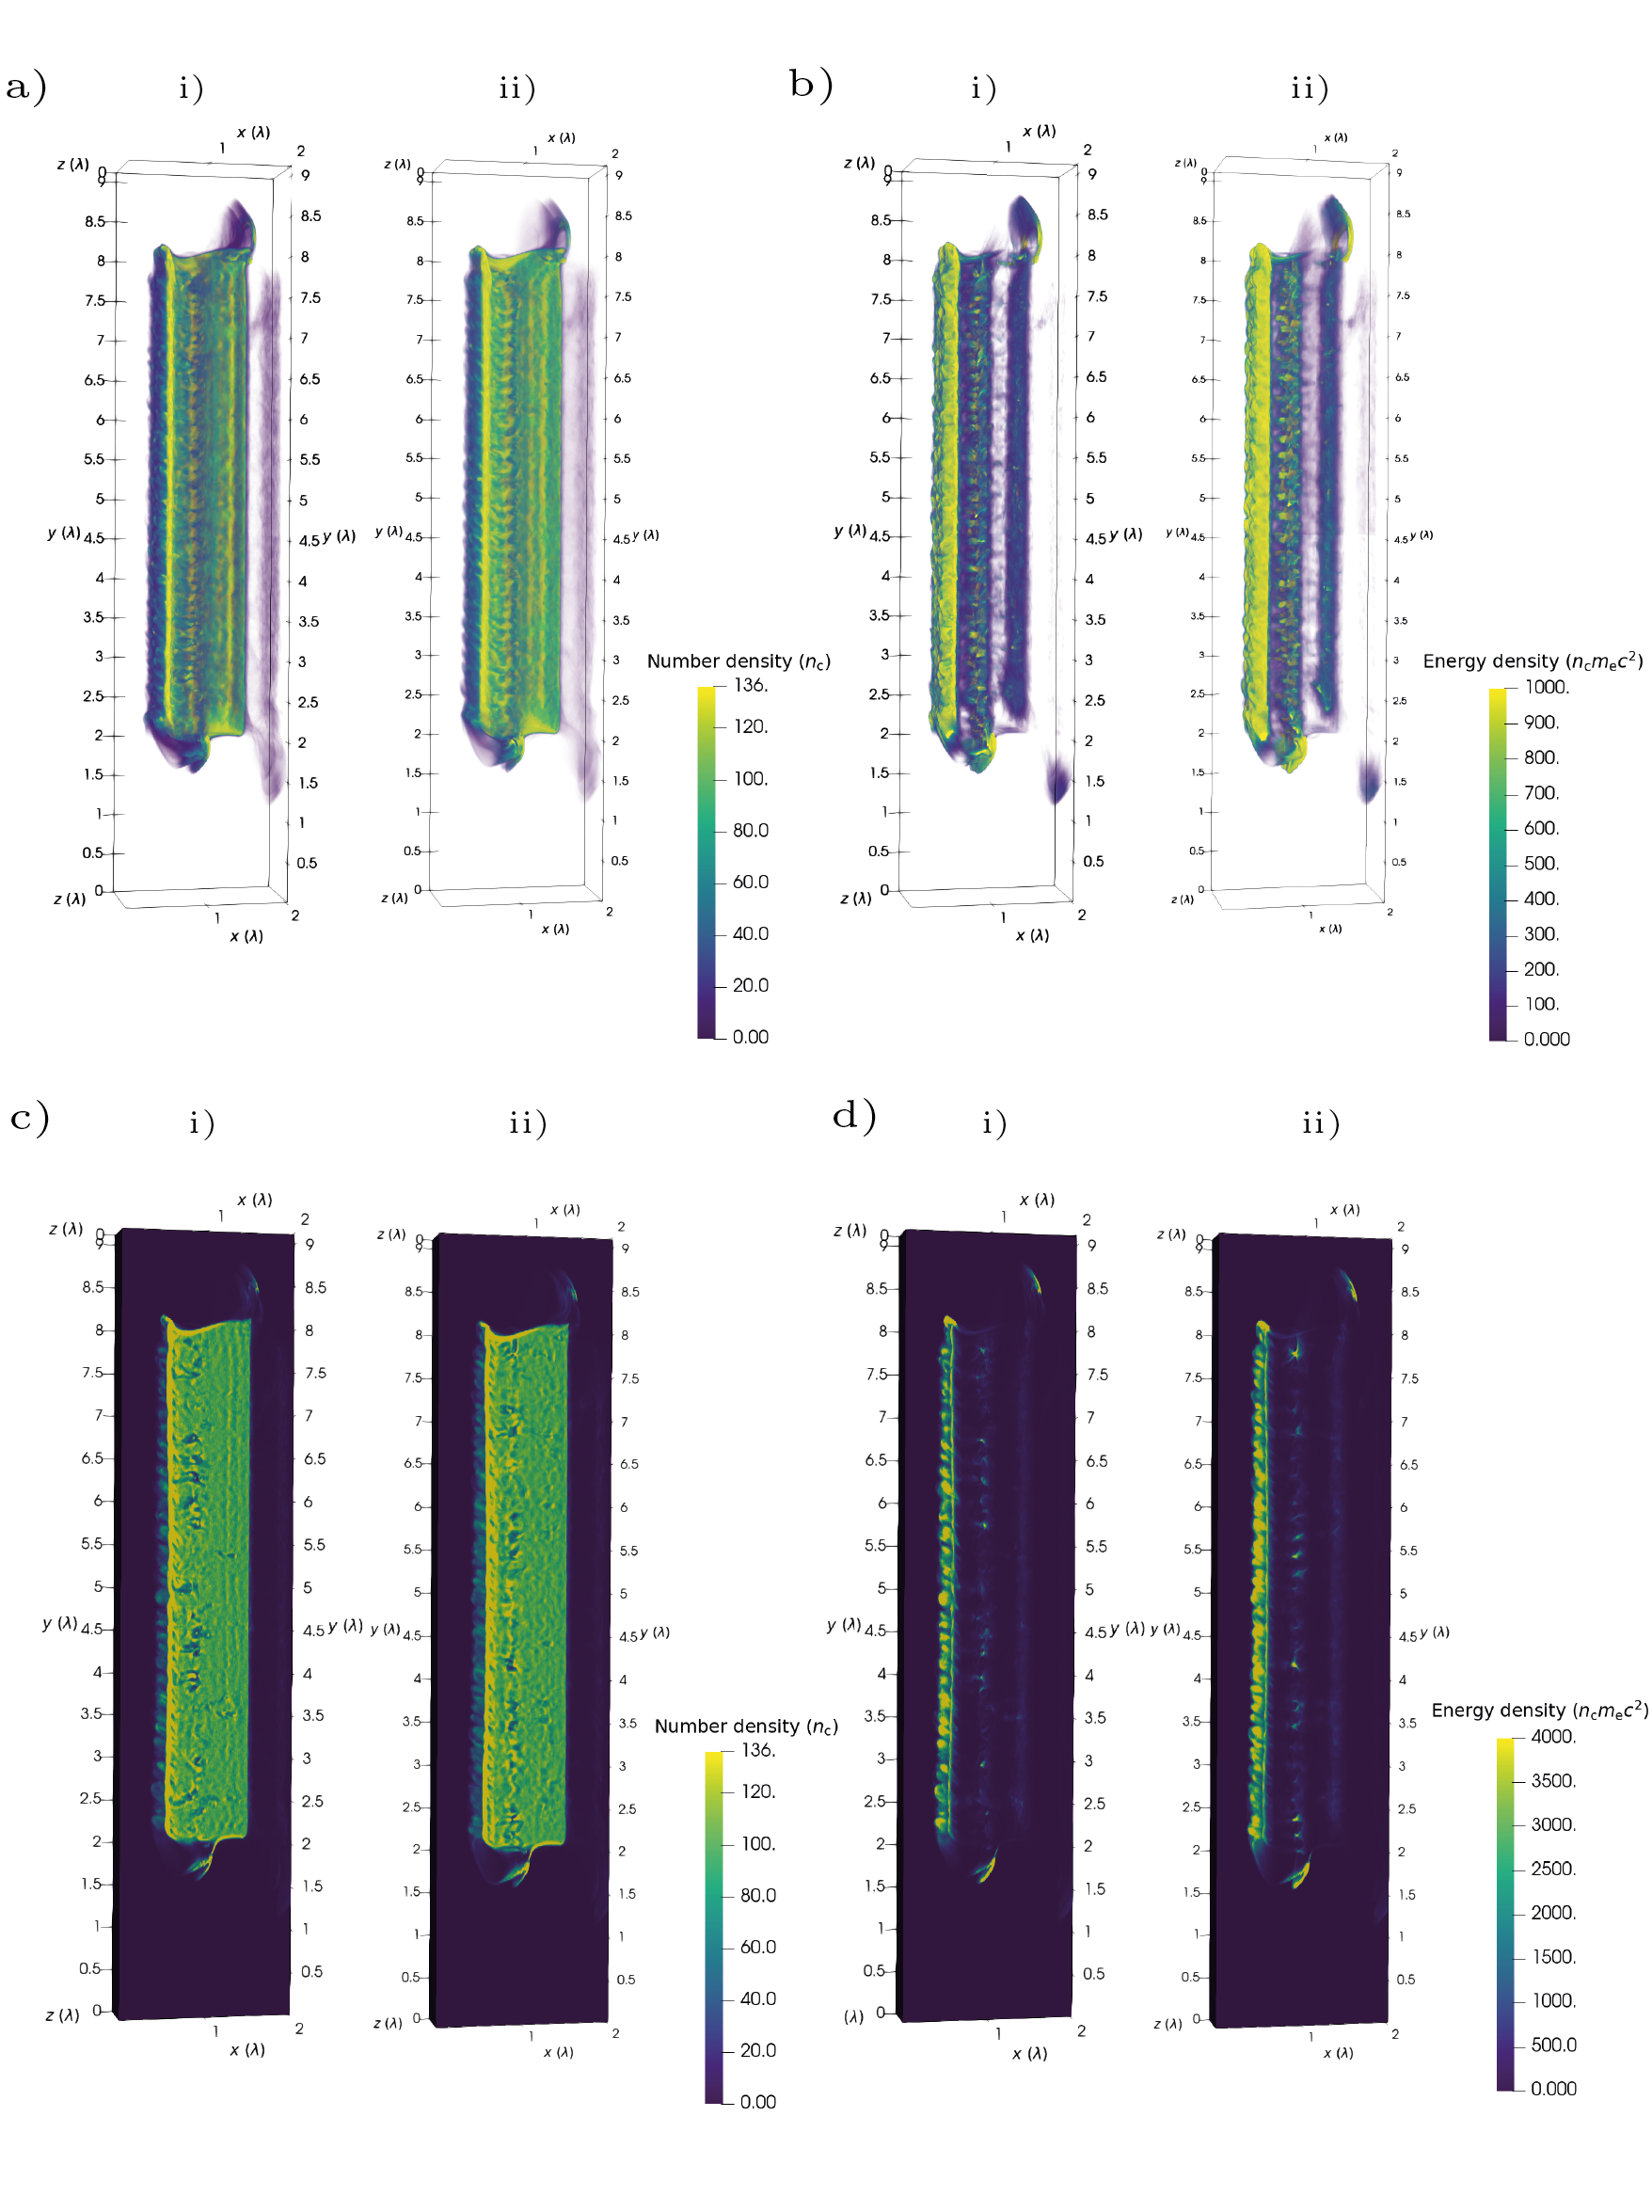
\includegraphics[width=1\linewidth]{figures/zvp/zvp_3D_compare_lowres}
	\caption[Comparison between the initial 3D simulation and a lower resolution version.]{Comparison between the initial 3D simulation and a lower resolution version. a) Electron number density. b) Kinetic energy density. c) and d) are slices of a) and b) respectively. $i$) Initial simulation. $ii$) Lower resolution simulation. Good convergence is demonstrated.}
	\label{fig:zvp3dcomparelowres}
\end{figure}
The two simulations are compared in figure \ref{fig:zvp3dcomparelowres}. Good convergence is qualitatively demonstrated by the presence of characteristic features of the ZVP mechanism. While the instabilities are similar in structure, the change in seeding changes their exact positions. As instabilities are not the focus of this thesis this variation is of no concern.


Maybe mention somewhere that I would als add pseudocapacitor field as an essential characteristic of the ZVP mechanism that should generally be identified.

Following the success in reproducing the key features of the \ac{ZVP} mechanism and demonstrated consistency between 2 and 3D equivalent simulations, the remainder of this chapter will predominantly utilise 2D simulations to interrogate the mechanism further.
\subsection{The ZVP electron bunch}
 Although much has been stated of the high energy and short duration of ZVP electron bunches in the previous work, until now much of the quantitative discussion of the properties of such bunches has avoided interrogation. A ZVP electron bunch is an electron bunch produced via the ZVP mechanism. Once produced and accelerated across the pseudocapacitor field, it is launched back in the laser propagation direction. While the bunch has no spatial separation over energies when propagating with the zero of the vector potential, the turning point of the electrons is longitudinal momentum dependent due to the Coulomb attraction of the ions after overshooting the pseudocapacitor field. Baeva \textit{et al} showed that the electron bunch has a quasi-monoenergetic spectrum: there is a one-to-one relationship between energy and position with the higher energies trailing the lower energies. The full bunch is confined to 130 as while a single energy confined to 5 as. If, however, the plasma bulk is transversely mass-limited relative to the laser spot size,when rotated back towards the plasma block, some of the electron bunch will overshoot and escape the potential well without significant stretching of the bunch in time as can be seen in figure \ref{fig:zvp3d}. Such electron bunches (retain the initial energy spread???? ie fast first as disucssed in RES paper) retain their high charge density and ultra-short duration. ZVP electron bunches can therefore be placed into two categories: ultra-high charge, ultra-short duraction electron bunches from mass-limited targets, hereafter labelled mass-limited electron bunches, of interest due to their unique properties and bulk propagating bunches, hereafter labelled bulk bunches, which have lower charge densities, are imprinted with instabilities and are instead of interest due to their connection to energy absorption and reflection in this post-ponderomotive regime.
 
 To investigate these two bunch types further, 2D PIC simulations were performed, see appendix for parameters. Figure blah is reprentative.
 
 \subsubsection{Attosecond nano-Coulomb mass-limited electron bunches}
 Figure \ref{fig:zvptypicalbunch} describes a typical mass-limited ZVP electron bunch qualitatively.
% TODO: \usepackage{graphicx} required
\begin{figure}
	\centering
	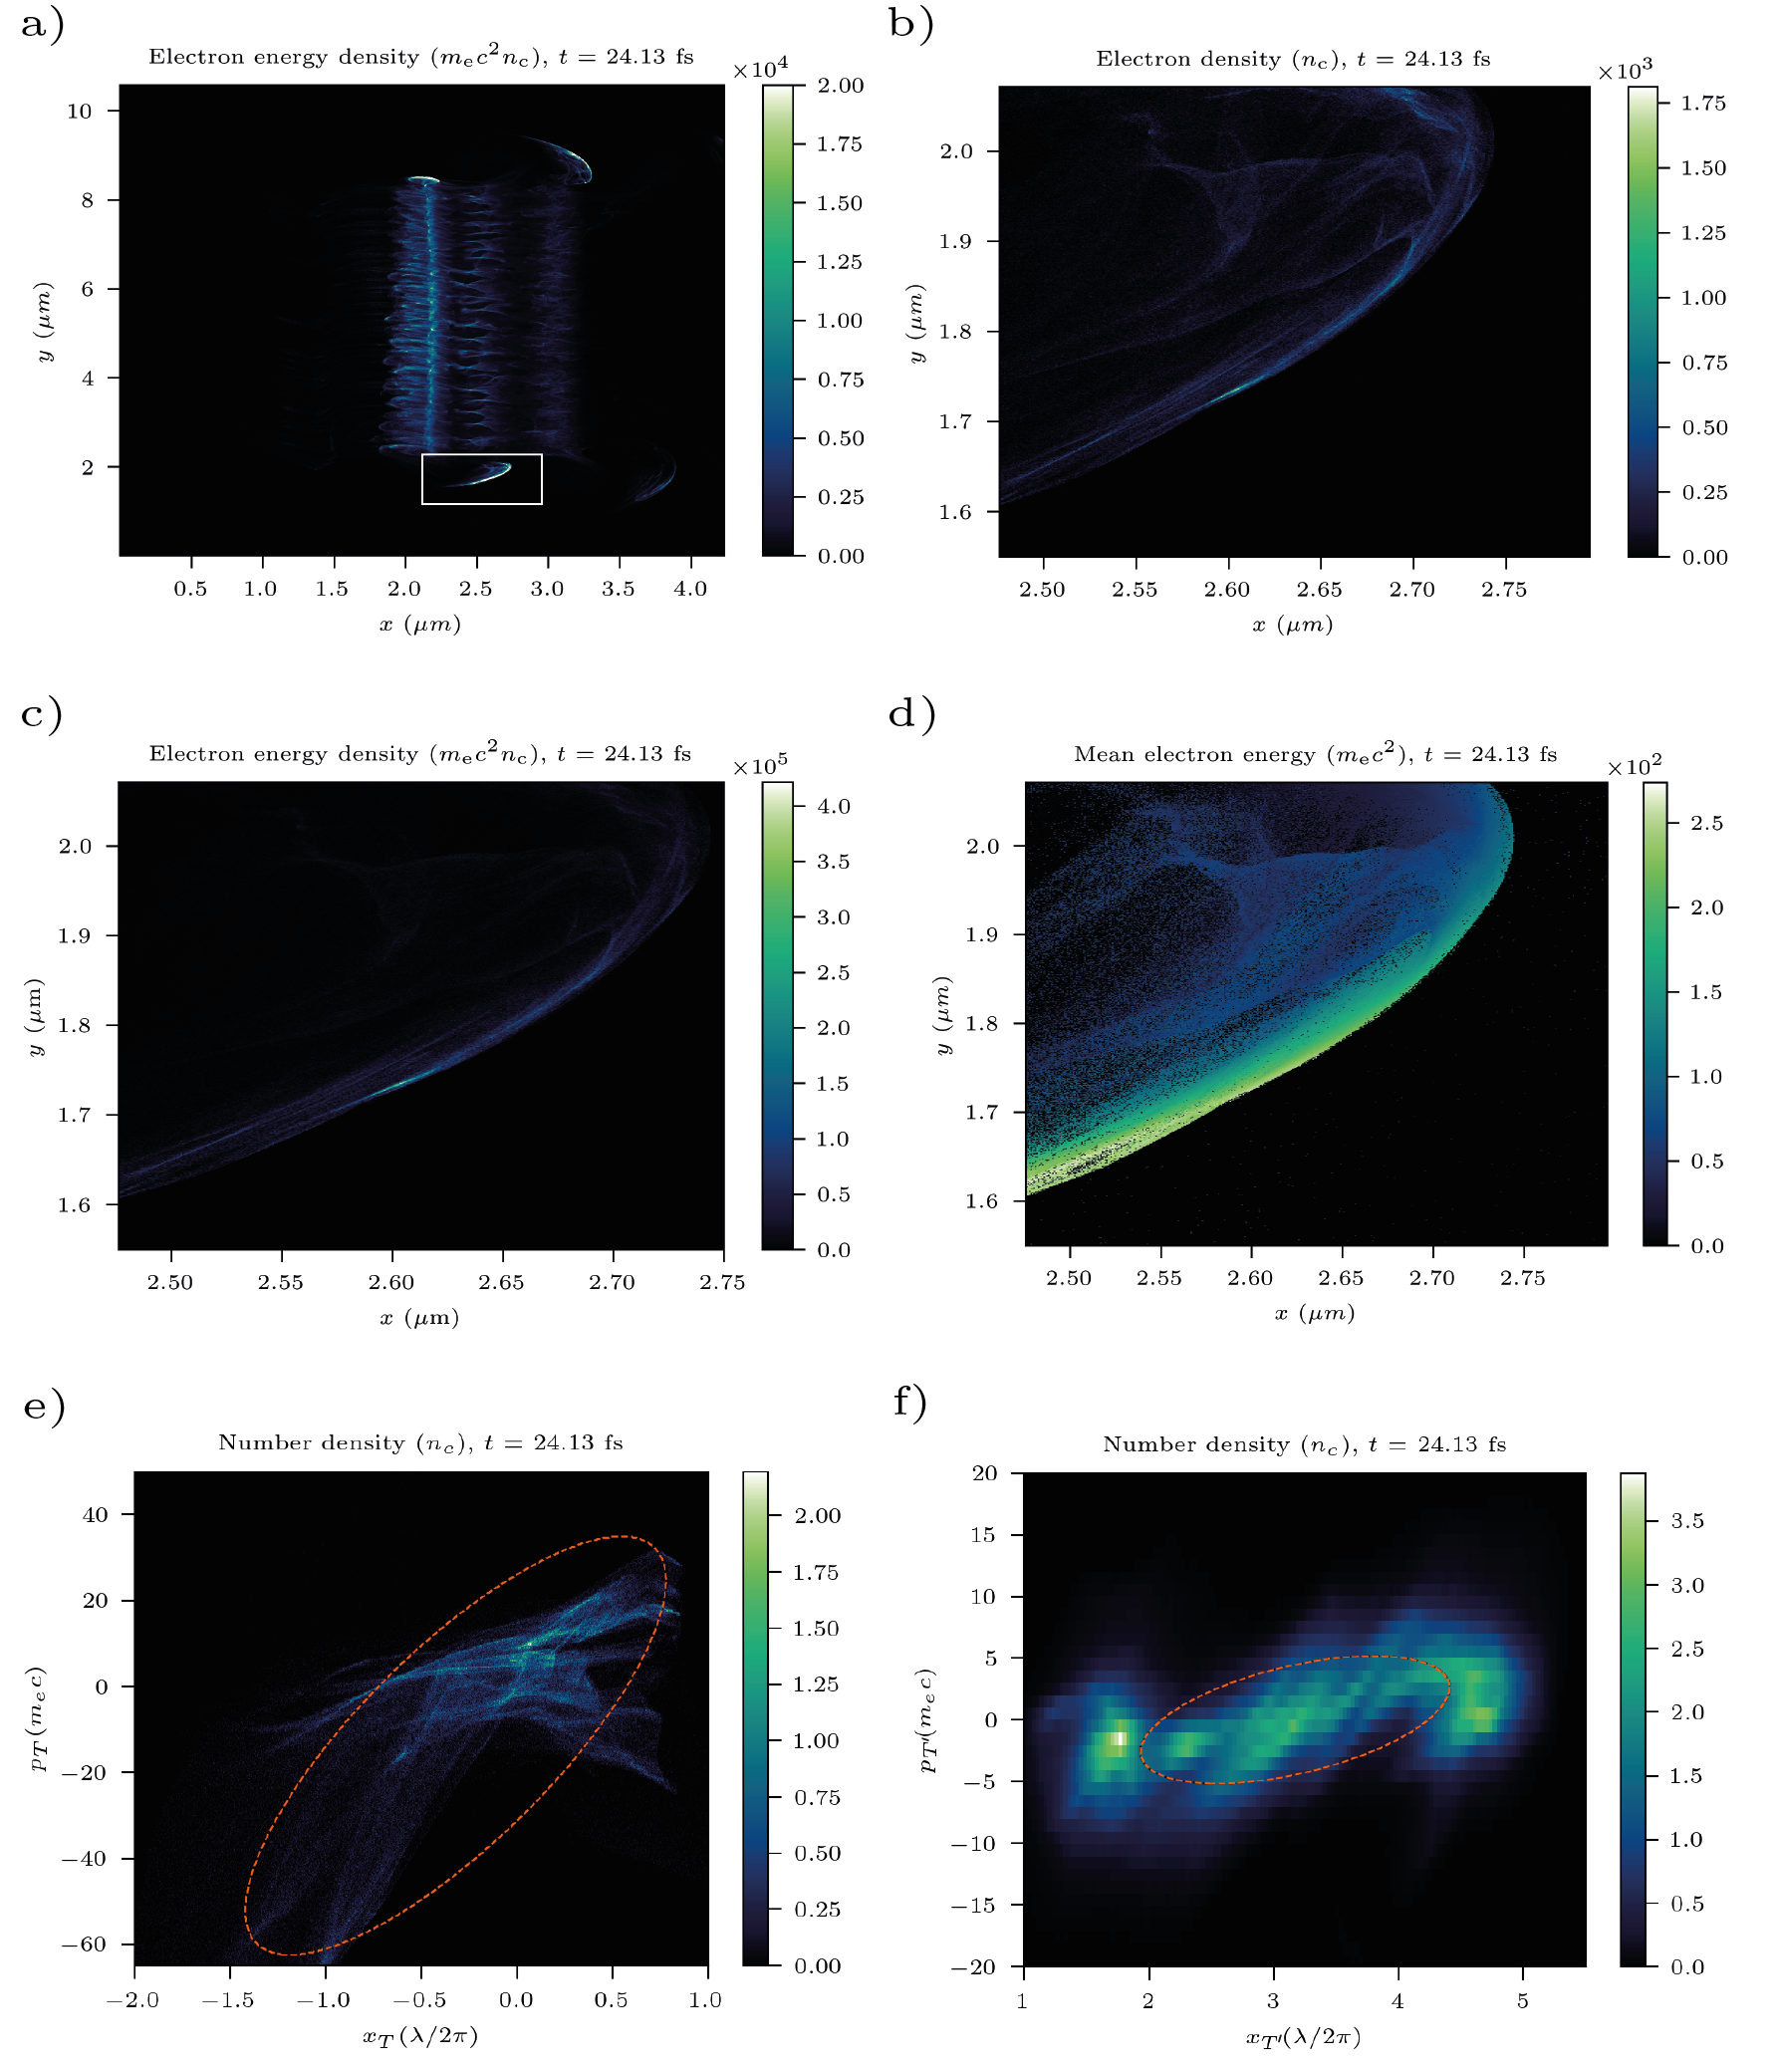
\includegraphics[width=1\linewidth]{figures/zvp/zvp_typical_bunch}
	\caption[2D PIC simulation results qualitatively describing typical mass-limited ZVP electron bunch structure.]{2D PIC simulation results qualitatively describing typical mass-limited ZVP electron bunch structure. a) Electron energy density for the full simulation window, corresponds to figure \ref{fig:zvp3d}f).  The box highlights the bunch presented in the following plots. b) Electron number density of the electron bunch. c) Electron energy density of the electron bunch, the colourbar scale has been increased compared to figure a) to demonstrate the internal structure. d) The mean electron energy across the electron bunch, suggesting a position dependent energy or quasi-monoenergetic nature to the electron bunch \cite{baevaZeroVectorPotential2011}. Cells with no macroparticles are black. e) The transverse phase space in the 2D simulation plane. The ellipse describes the calculated emittance. The skew of the ellipse is a consequence of a low density tail on the phase space beyond the bottom left corner. f) This plot was extracted from the equivalent 3D simulation and describes the transverse emittance in the $z$-direction. Again the ellipse marks the emittance. The relatively well-defined border to the phase space and the mild tilt (indicating only mild divergence) are direct consequences of the 2D nature of the interaction.}
	\label{fig:zvptypicalbunch}
\end{figure}
The electron bunch under interrogation is ultra-relativistic with a mean energy of \qty{51\pm 11}{MeV} and a duration of 35 as. It propagates at an angle of -393 rad relative to the laser propagation direction, \textit{i.e.} the $x$-axis, and a transverse geometric emittance in the simulation plane (the $x$-$y$ plane) of \qty{35 \pm 7}{nm.rad}. A definition of the transverse geometric emitance, a measure of the quality of the electron beam, is given in appendix \ref{app:1-basics-transverse_emittance}. Note that while the bunch does not propagate in the laser propagation direction, this does not mean it must be rejected under consideration of the ZVP bunch conditions. Indeed, the bunch must propagate at some angle to the laser since conservation of canonical momentum while it remains in thrall of the laser pulse it must have some transverse component of momentum. The more standard ZVP bunches passing through the bulk again by conservation of momentum must propagate along the axis, as is observed in simulation. For an equivalent bunch in a corresponding 3D simulation, the transverse geometric emittance in the $z$ plane is \qty{15\pm 11}{nm.rad}. This electron bunch has a total charge of 0.35 nC for a slab of plasma of thickness $0.75\lambda$ in the $z$-direction. Noting again the two-dimensional nature of the interaction geometry, and that electrons less than twice the relativistic Larmor radius, 
\begin{equation}
	r_\mathrm{l} = \frac{\gamma m_\mathrm{e}v}{eB},
\end{equation}
where $\gamma$ and $v$ correspond to the electron velocity and $B$ is the magnetic field of the laser pulse, when rotated back towards the plasma will escape to the side, the total number of electrons in the mass-limited bunch is
\begin{equation}
	N = 2 n_\mathrm{e} r_\mathrm{l} L_z \Delta x,
\end{equation}
where $L_z$ is the width of the plasma in the $z$-direction. Using equation \ref{eq:zvp_dx} for $\Delta x$ and \ref{eq:zvp_gamma} for $\gamma$ and approximating $v \approx c$ for the ultra-relativistic electron bunch, 
\begin{equation}\label{eq:zvp_N}
	N = 2 \gamma n_\mathrm{c} \frac{L_z}{k^2}.
\end{equation}
For these simulation parameters, this corresponds to a total bunch charge, $Q = eN$, of 0.37 nC, a remarkably successful prediction of the ZVP model. Equation \ref{eq:zvp_N} tells us there is no limit to the 

Equation \ref{eq:zvp_N} can be rewritten in terms of fundamental constants as
\begin{equation}\label{eq:zvp_N2}
	N = 2 (1+0.5\frac{a^2_0}{\bar{n}_\mathrm{e}}) L_z \frac{m_\mathrm{e}\epsilon_0c^2}{e^2}.
\end{equation}
Almost counterintuitively, it would appear the total charge scales inversely with the plasma density. Instead, charge can be increased either by increasing the laser pulse intensity or $L_z$. Indeed, provided the laser pulse intensity remains relativistic, the focal spot can be increased indefinitely and there is no limit to the mass-limited electron bunch total charge. For a realistic laser pulse with beam width $10 \lambda$ incident on a larger laser block, equation \ref{eq:zvp_N2} predicts a charge of 9.3 nC.


Discuss use cases of the electron bunches.
DIscuss if  bunch quasi-monoenergetic.

Figure blah blah compares the electorn bunch energy to an equivalent\footnote{A circularly polarised laser pulse will expel electrons from a mass-limited target in a corkscrew shape, the bunch is therefore only loosely equivalent.} bunch produced by a circularly polarised laser pulse. The mean electron bunch energy is over three times lower as there is no ZVP acceleration phase and there is no quasi-monochromatic nature \cite{baevaZeroVectorPotential2011}. 

\subsubsection{Parameter scan of electron bunch mean energy}
Since ZVP energy scaling is a fundamental identifier of ZVP bunches, it is important to confirm that mass-limited electron bunches follow the same scaling relations as has previously been confirmed for bulk ZVP electrons in both 1D \cite{baevaZeroVectorPotential2011} and 2D \cite{savinAttosecondscaleAbsorptionExtreme2017} PIC simulations. The mean mass-limited electron bunch kinetic energies were extracted from 120 2D PIC simulations and are plotted in figure \ref{fig:zvpmeangammas}. 
% TODO: \usepackage{graphicx} required
\begin{figure}
	\centering
	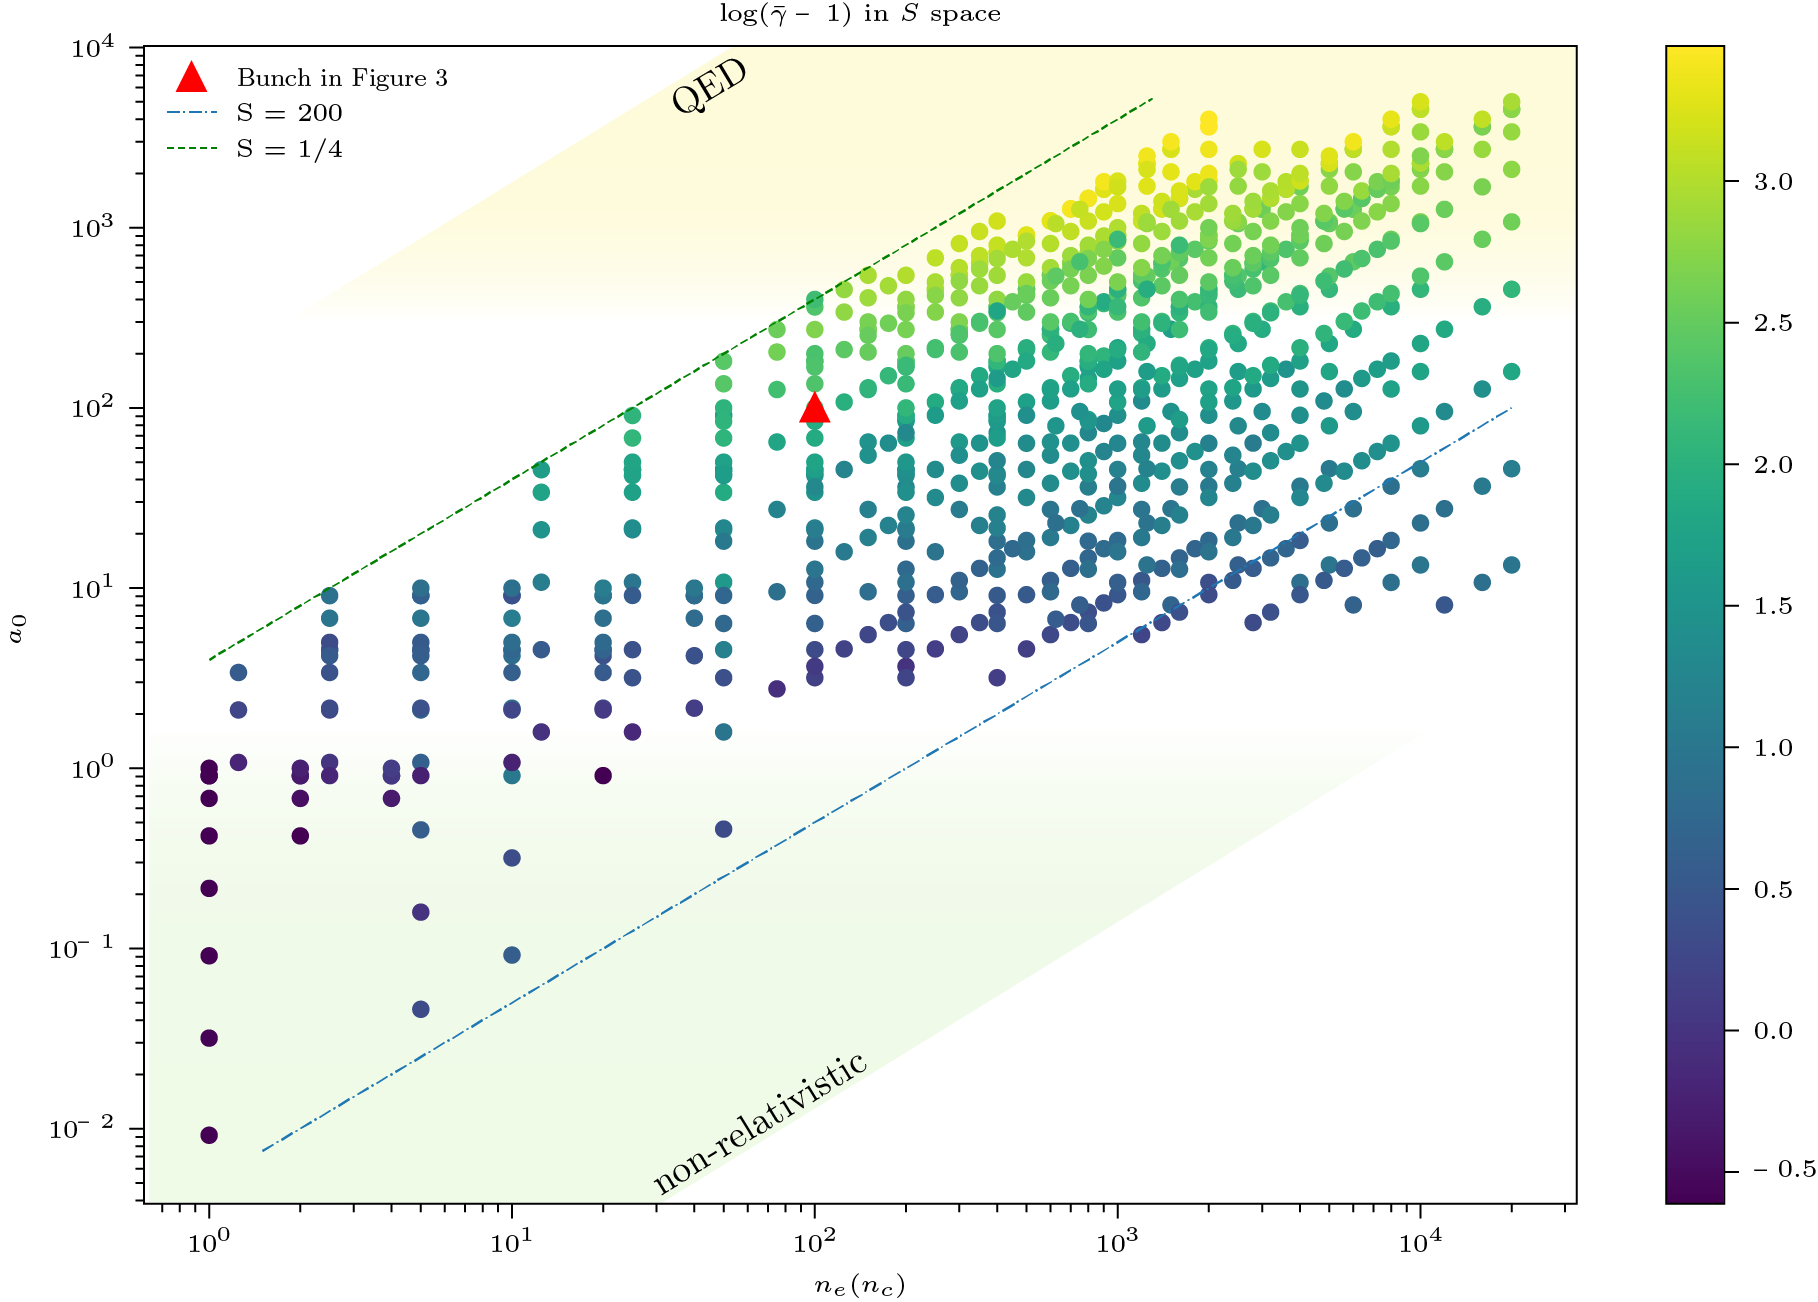
\includegraphics[width=1\linewidth]{figures/zvp/zvp_mean_gammas}
	\caption[Mean mass-limited ZVP electron bunch normalised kinetic energies extracted from 2D PIC simulations.]{Mean mass-limited ZVP electron bunch normalised kinetic energies extracted from 2D PIC simulations. The bunch detailed in figure \ref{fig:zvptypicalbunch} is highlighted.}
	\label{fig:zvpmeangammas}
\end{figure}
The dependence on both $a_0$ and $n_\mathrm{e}$ demonstrates these electron bunches are accelerated by a non-pondermotive mechanism. The parameter scan ranged plasma block density ranging from the critical plasma density to well-beyond solid density for the aluminium target and with laser pulse peak intensity ranging from non-relativistic ($a_0 < 1$) through to the \ac{QED} plasma regime ($a_0 > 300$) up to a peak $a_0 = 5000$ to investigate the change in scaling observed by Savin \textit{et al} \cite{savinEnergyAbsorptionLaserQED2019} at the onset of QED effects. This study is also the first to extract specific bunch energies as opposed to total simulation box energy gain, representing a far more stringent test of ZVP theory.

Care must be taken however as the energy of such electron bunches cannot be directly compared to the ZVP energy relations as as aforementioned after escaping the potential, the electron bunch experiences further direct laser acceleration before reaching the detection point. Indeed, Thévenet \textit{et al} \cite{thevenetVacuumLaserAcceleration2016} suggested that attosecond electron bunches produced in reflection exhibit precisely the phase and energy properties required to `surf' the reflected laser pulse and experience vast acceleration gradients over the Rayleigh length of the laser pulse. This process is known as Vacuum Laser Acceleration. It seems highly likely that this process occurs for electron bunches produced in transmission. This seemingly unfortunately situation in reality provided a fully optical scheme to create GeV nano-Coulomb electron bunches from the most simple of setups: a laser interacting with a mass limited solid target (thus reducing the alignment complexity.). 

Returning to the determination of the electron bunch energy at the measurement point, consider now the journey of the electron bunch after expulsion from the plasma bulk. It is rotated back towards the plasma bulk by the magnetic field of the subsequent peak of the laser pulse, then travelling at approximately $c$ it surfs the peak, experiencing an approximately constant accelerating electric field from the laser pulse at some fraction $f$ of the laser field peak. The work done by this field is then
\begin{equation}
	\Delta T = \int e \mathbf{E} \cdot \mathrm{d}\mathbf{x}.
\end{equation}
Note that for this process, the laser pulse electric field and electron bunch direction of travel will always be aligned no matter to which side of the plasma bulk the electrons are accelerated to and therefore $\Delta T$ will always increase the energy of the electron bunch, thus,
\begin{equation}
	\Delta T = e f E_\mathrm{L} \Delta y,
\end{equation}
where $\Delta y$ is the distance along $y$ from the plasma edge to the detection point. Accounting for the Gaussian spatial profile of the laser, $a(t) = a_0 \exp(-y^2/(6\lambda)^2)$ at focus, the gamma factor after both acceleration phases for this simulation setup is then
\begin{equation}\label{eq:zvp-gamma}
	\gamma = 1 + (0.30)\times \frac{a^2_0}{\bar{n}_\mathrm{e}} + (1.2f)\times a'_0.
\end{equation}
Here the primed vector potential refers to the intensity of the subsequent peak of the laser pulse. This final term could be neglected or at least reduced somewhat once super-Gaussian spatial laser pulses become standard in this intensity regime or using a suitable plasma separator \cite{miyauchi_2004_LaserElectronAcceleration}. Both acceleration phases fail to meet the criteria of the Lawson-Woodward theorem. The ZVP phase is dependent on the existence of electrostatic forces, while the secondary phase occurs for a finite interaction region.

Fitting equation \ref{eq:zvp-gamma} to the PIC simulation data presented in figure \ref{fig:zvpmeangammas} finds
\begin{equation}
	\gamma = 1 + (0.46\pm 0.02)\times \frac{a^2_0}{\bar{n}_\mathrm{e}} + (0.28\pm 0.01)\times a'_0
\end{equation}
with an $r^2$-value of 0.818. This fit suggests $f = 0.22\pm 0.01$. The electric field experienced for a random selection of electrons in a bunch was extracted from one simulation. Encouragingly, the mean attenuation of the electric field they experience is $0.20\pm0.05$, to calculate this attenuation directly falls beyond the scope of ZVP theory.

This is the first demonstration of ZVP theory to calculate actual values and not only the scaling relationship. Such order of magnitude calculation is essential to compare this model of absorption to others and thus determine the dominant mode for absorption. It is certainly remarkable that such a simple theory for energy absorption has such predictive success in this highly non-linear and seemingly chaotic many particle system. It is interesting that increasing laser intensity to such extremes will, at least for a short time, cause relativistic effects that add coherency to electron motion before total annihilation of a target.

The relative error between data and theory is plotted in figure \ref{fig:zvp-logabserrortedit}. 
% TODO: \usepackage{graphicx} required
\begin{figure}
	\centering
	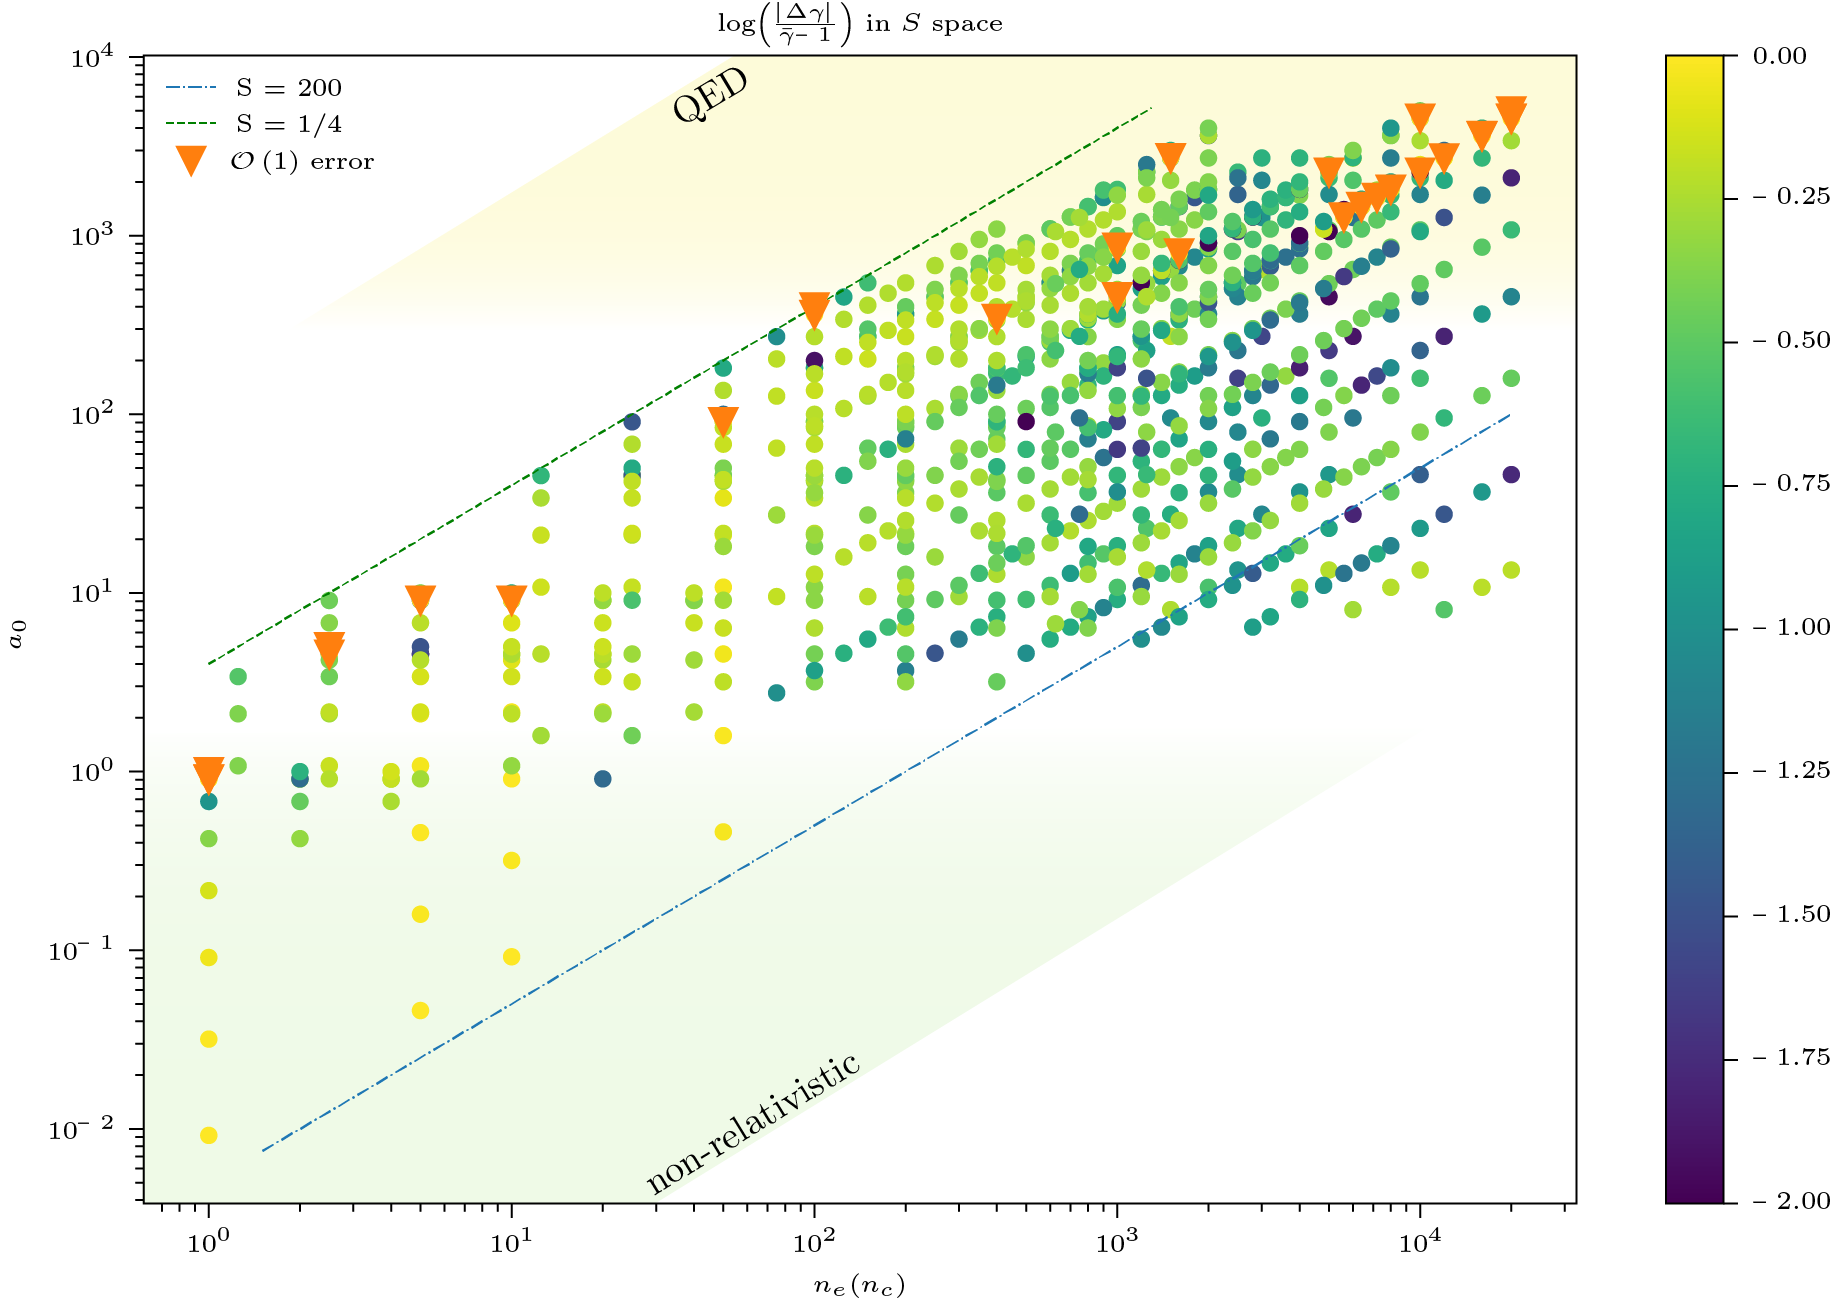
\includegraphics[width=1\linewidth]{figures/zvp/log_abs_error_T_edit}
	\caption[The relative errors for each mean energy data point compared to figure \ref{fig:zvpmeangammas}.]{The relative errors for each mean energy data point compared to figure \ref{fig:zvpmeangammas}. The orange triangles indicate data points for which the model fails to predict the mean energy.}
	\label{fig:zvp-logabserrortedit}
\end{figure}
Those points marked by an orange triangle have associated errors of over an order of magnitude. Reassuringly, such points occur only after the onset of QED effects, known to impact the ZVP mechanism \cite{savin_2019_EnergyAbsorptionLaserQED} and for $S<1$, that is, where the plasma becomes relativistically transparent to the laser pulse, a fundamentally different regime. Equally, for non-relativistic laser intensities, where assumptions of electron coherency cannot be made, are poorly fit by the model. It is particularly interesting that there is no indication that large $S$ causes a breakdown of the model, extending the applicability of the model further than previously considered, opening up the field to a wider range of conditions, such as that of shock compressed plasmas. To summarise, it would appear the ZVP model is valid for $10 \le a_0 \le 300$ and $S\ge1$.



To do:
Look again at trajectories
Look again at just fitting the region where expression is valid.
Temporal effects (non-existant, discuss)


\subsection{Energy absorption in the ZVP regime}\label{sec:zvp-energyabsorption}
As stated previously the laser-plasma coupling exists in a state of adiabaticity with the exception of the ZVP acceleration phase and hence equation \ref{eq:zvp_U} describes the absorption of laser pulse energy. For normal incidence, the rate of energy transfer is therefore
\begin{equation}\label{eq:zvp-rate}
	R = \frac{U\omega_\mathrm{L}}{\pi},
\end{equation}
since two bunches are produced per laser cycle. To demonstrate the scaling for $U$ in 2D PIC simulations, peak instantaneous electron bunch energies escaping to the rear of the bulk were extracted from those PIC simulations with $S=1$. For constant $S$, 
\begin{equation}
	U \sim a^2_0.
\end{equation}
Eneriges are plotted in figure \ref{fig:zvppeakgamma}.
% TODO: \usepackage{graphicx} required
\begin{figure}
	\centering
	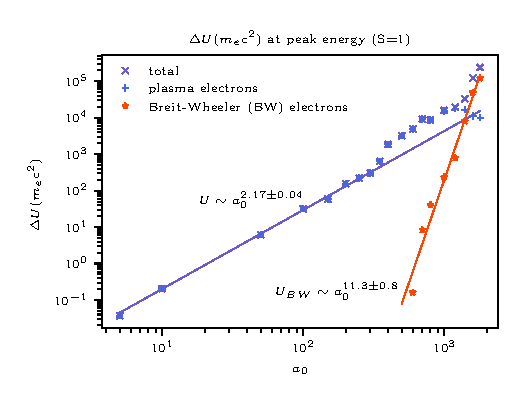
\includegraphics[width=0.7\linewidth]{figures/zvp/zvp_peak_gamma}
	\caption[Peak instantaneous bulk electron bunch total energy escaping to the plasma bulk rear.]{Peak instantaneous bulk electron bunch total energy escaping to the plasma bulk rear.}
	\label{fig:zvppeakgamma}
\end{figure}
Fitting the total energy within the range of validity established for the ZVP model finds
\begin{equation}
	U \sim a^{2.01\pm0.003}_0,
\end{equation}
reproducing with great success the anticipated scaling within the ZVP regime. It is also quite satisfying that the number of electrons and bunch mean energies both follow their anticipated ZVP scalings, further evidence this is not a simple ponderomotive effect. By extracting specific bunch total energies, rather than just the peak energies of the plasma block as a whole as was performed in previous studies, this is a far more direct confirmation of energy absorption by the ZVP mechanism into electron bunches. This is highlighted by the difference in results obtained for this study compared to a previous study by Savin \textit{et al} \cite{savin_2019_EnergyAbsorptionLaserQED} when investigating the QED regime as will be discussed later. It was not possible to reproduce the constants of equation \ref{eq:zvp_U} as the neutralising return current in the plasma bulk generates an electrostatic field on the rear side of the plasma block, decelerating bulk electron bunches as they escape the plasma. It should be possible to calculate the deceleration by considering the number of electrons expelled by the plasma. It is however, clear from the simulations that at least some electrons in the escaping bunch are trapped by this rear-side potential well reducing its magnitude.

While equation \ref{eq:zvp_U} describes energy absorption into hot electron bunches, the coupling of such hot collisionless electrons to the bulk plasma given the lack of collisionality is necessarily indirect. There are two key mechanisms \cite{sherlock_2014_IndepthPlasmawaveHeating}. Firstly, via a cooler resistive return current of electrons that neutralises the current of the injected hot electrons that escape the potential well of the front surface (cite this, the refernce in sherlock 2014 is not great). Since all hot electrons travel at approximately speed $c$, the magnitude of the return current depends not on the total energy absorbed but instead on the total number of electrons injected, as given by equation \ref{eq:zvp-Ne}, depending linearly on laser spot area and the electric field magnitude and not on the plasma density\footnote{Note that for a sufficiently thin target, the return current induces an electrostatic field on the back surface of the target which can then reflect hot electron bunches and decelerate them to the point of a return to collisionality. This is a reality for the PIC simulations explored in this thesis, however, since realistic targets are much thicker this shall be neglected.}. Secondly, via the formation of large amplitude bulk plasma waves induced in the wake of the hot electron bunches. Sherlock \textit{et al} \cite{sherlock_2014_IndepthPlasmawaveHeating} calculate the magnitude of the induced wakefield to be
\begin{equation}
	E_\mathrm{W} = \frac{eN_\mathrm{e}c}{\omega_\mathrm{p}\epsilon_0} = \sigma \sqrt{\frac{m_\mathrm{e}\epsilon_0}{n_\mathrm{e}}}E_\mathrm{L},
\end{equation}where here the bunch velocity has been set to $c$, bulk electrons will be accelerated by $E_\mathrm{W}$ and their kinetic energy converted to heat via collisions. Interestingly, this reproduces the mid temperature electon scaling with density that was observed by Chrisman \textit{et al} \cite{chrisman_2008_IntensityScalingHot} in their study of hot electron energy coupling in cone-guided fast ignition of inertial fusion targets. This is a significantly different possible explanation to their self-declared 'hand waving argument'. Excluding this study, such formulations for heat transfer to the plasma bulk within the ZVP regime remain untested in simulations.


Note also that as the laser pulse intensity rises, the fraction of energy absorbed by the ion species increases. Savin \cite{savin_2019_ModellingLaserPlasmaInteractions} determined for $S=1/2$, $a_0 = 100$, that this would be almost 20\%. Energy is absorbed by ions via the hole boring mechanism as described elsewhere in this thesis.


\subsection{Unpacking the QED effects of figure \ref{fig:zvppeakgamma}}
In Savin's influential paper \cite{savin_2019_EnergyAbsorptionLaserQED}, he determined theoretically and demonstrated in simulation that at $a_0 = 300$, $n_\mathrm{e} = 50 n_\mathrm{c}$, there is a transition from standard ZVP scalings to an enhance QED scaling associated with \ac{BW} electrons increasing the pseudocapacitor plate charge. Explicitely,
\begin{equation}
	T \sim \frac{a^5_0}{\bar{n}_\mathrm{e}}.
\end{equation}
Such a scaling shift was not observed for the large parameter scan presented in figure \ref{fig:zvpmeangammas}. Simulations revealed this was likely due to few \ac{BW} pairs produced towards the plasma edges and hence no additional gain in energy from crossing the pseudocapacitor. Another concern is Savin's study was conducted within the regime of relativistic transparency where it is unclear whether the ZVP potential well can be maintained and was not explored in this study. The final consideration is the well known effect of radiation trapping due to the radiation reaction \cite{jiRadiationReactionTrappingElectrons2014}, also observed in these PIC simulations. After acceleration across the pseudocapacitor, the electron bunch encounters the subsequent laser peak. If the electron bunch gamma factor and laser intensity are both large enough (include chi requirement), electrons radiate a significant fraction of their energy and are thus stopped in their tracks. Unable to now escape the potential well at the plasma surface they remain trapped and are not observed to escape the plasma until the laser pulse intensity reduces. Such an effect would not impact Savin's scalings but would of course inhibit the observation of the scaling for electrons escaping to the sides and rear of the plasma block.

Returning now to figure \ref{fig:zvppeakgamma}, there are two interesting aspects. Firstly the sudden jump in total energy at $a_0 \approx$ 300. This cannot be explained by ZVP theory nor QED theory since the jump is observed with QED effects switched off. 

Secondly, the even sharper jump in total electron bunch energy above $a_0 = 1000$. Decomposing the total energy into bulk electrons and those produced via the BW process, this is clearly a QED effect. Energy in BW pairs scales at a staggering
\begin{equation}
	U_\mathrm{BW} \sim a^{11.3\pm 0.8}_0,
\end{equation}
while energy in plasma electrons descreases. Perhaps this is a signal of Savin's QED ZVP electron bunches only at a higher energy due to the substantially greater plasma density of these simulations. Following Savin's theory,
\begin{equation}
	U_\mathrm{QED} \sim \frac{a^7_0}{S}.
\end{equation}


The reduction in plasma electron energy can be attributed to an oversaturation of the front surface with BW electrons. The surface now consists of mostly BW electrons. Could this replacement explain the increase in scaling observed vs the theory or can it be explained by radiation reaction or is there some other deeper effect at work?

Doubtless, the advent of next generation exa-watt scale lasers and the ability to explore this regime will be exceedingly interesting if such scalings in bunch energy can be maintained.


Discuss region of BW pair projection maximisation and where we expect saturation.

To do: Explore transition regions, do MORE simulations to fill in the gaps.


Then experiment?

Numerical heating: it is not sufficient to simply run simulations without the laser pulse to determine heating. The effect of numerical heating will be most damning for the ultra-high charge density electron bunches.

To do: convergence of electron bunch energies with nppc and sim resolution.


At aome point mention:

Note that ZVP does not describe the peak energies in the bunches, then JxB applies, since there are always some electrons outside of the well defined sharp boundary when the density is not high enough to impose adiabaticity. 
